    %%
%% This is file `sample-sigconf-authordraft.tex',
%% generated with the docstrip utility.
%%
%% The original source files were:
%%
%% samples.dtx  (with options: `all,proceedings,bibtex,authordraft')
%% 
%% IMPORTANT NOTICE:
%% 
%% For the copyright see the source file.
%% 
%% Any modified versions of this file must be renamed
%% with new filenames distinct from sample-sigconf-authordraft.tex.
%% 
%% For distribution of the original source see the terms
%% for copying and modification in the file samples.dtx.
%% 
%% This generated file may be distributed as long as the
%% original source files, as listed above, are part of the
%% same distribution. (The sources need not necessarily be
%% in the same archive or directory.)
%%
%%
%% Commands for TeXCount
%TC:macro \cite [option:text,text]
%TC:macro \citep [option:text,text]
%TC:macro \citet [option:text,text]
%TC:envir table 0 1
%TC:envir table* 0 1
%TC:envir tabular [ignore] word
%TC:envir displaymath 0 word
%TC:envir math 0 word
%TC:envir comment 0 0
%%
%% The first command in your LaTeX source must be the \documentclass
%% command.
%%
%% For submission and review of your manuscript please change the
%% command to \documentclass[manuscript, screen, review]{acmart}.
%%
%% When submitting camera ready or to TAPS, please change the command
%% to \documentclass[sigconf]{acmart} or whichever template is required
%% for your publication.
%%
%%
\documentclass[sigconf,authordraft]{acmart}
%%
%% \BibTeX command to typeset BibTeX logo in the docs
\AtBeginDocument{%
  \providecommand\BibTeX{{%
    Bib\TeX}}}

%% Rights management information.  This information is sent to you
%% when you complete the rights form.  These commands have SAMPLE
%% values in them; it is your responsibility as an author to replace
%% the commands and values with those provided to you when you
%% complete the rights form.
\setcopyright{acmlicensed}
\copyrightyear{2018}
\acmYear{2018}
\acmDOI{XXXXXXX.XXXXXXX}
%% These commands are for a PROCEEDINGS abstract or paper.
% \acmConference[Conference acronym 'XX]{Make sure to enter the correct
%   conference title from your rights confirmation email}{June 03--05,
%   2018}{Woodstock, NY}
\acmConference[CS 588]{Data Science For Software Engineering}{Fall 2025-26}{Bilkent University}
%%
%%  Uncomment \acmBooktitle if the title of the proceedings is different
%%  from ``Proceedings of ...''!
%%
%%\acmBooktitle{Woodstock '18: ACM Symposium on Neural Gaze Detection,
%%  June 03--05, 2018, Woodstock, NY}
\acmISBN{978-1-4503-XXXX-X/2018/06}

\usepackage{xcolor}
\usepackage{hyperref}
\usepackage{fontawesome}
%%
%% Submission ID.
%% Use this when submitting an article to a sponsored event. You'll
%% receive a unique submission ID from the organizers
%% of the event, and this ID should be used as the parameter to this command.
%%\acmSubmissionID{123-A56-BU3}

%%
%% For managing citations, it is recommended to use bibliography
%% files in BibTeX format.
%%
%% You can then either use BibTeX with the ACM-Reference-Format style,
%% or BibLaTeX with the acmnumeric or acmauthoryear sytles, that include
%% support for advanced citation of software artefact from the
%% biblatex-software package, also separately available on CTAN.
%%
%% Look at the sample-*-biblatex.tex files for templates showcasing
%% the biblatex styles.
%%

\usepackage{tikz}
\usepackage{pgfplots}
\usepackage{clipboard}
\newclipboard{manuscript}

% Revised macro for auto-sync with response letter
\newcommand{\revised}[2]{%
    % A. GÖRSEL KISIM: Metni PDF'e mavi renkte basar
    \textcolor{blue}{#2 (Reviewers #1)}%
    %
    % B. MANTIKSAL KISIM: Her ID için clipboard'a kopyalar
    \renewcommand{\do}[1]{%
        \label{rev:##1}%
        \setbox0=\vbox{%
            \Copy{text:##1}{#2}%
        }%
    }%
    \docsvlist{#1}%
}
%%
%% The majority of ACM publications use numbered citations and
%% references.  The command \citestyle{authoryear} switches to the
%% "author year" style.
%%
%% If you are preparing content for an event
%% sponsored by ACM SIGGRAPH, you must use the "author year" style of
%% citations and references.
%% Uncommenting
%% the next command will enable that style.
%%\citestyle{acmauthoryear}


%%
%% end of the preamble, start of the body of the document source.
\begin{document}

%%
%% The "title" command has an optional parameter,
%% allowing the author to define a "short title" to be used in page headers.
\title{Graph Enhanced Transformer for Semi-Supervised Duplicate Bug Report Detection}

%%
%% The "author" command and its associated commands are used to define
%% the authors and their affiliations.
%% Of note is the shared affiliation of the first two authors, and the
%% "authornote" and "authornotemark" commands
%% used to denote shared contribution to the research.
\author{Kerem Bayramo\u{g}lu}
\authornote{Authors are listed in alphabetical order by surname.}
\authornotemark[0]
\email{kerem.bayramoglu@bilkent.edu.tr}
\affiliation{%
 \institution{Bilkent University}
 \institution{Dept. of Computer Engineering}
 \city{\c{C}ankaya}
 \state{Ankara}
 \country{T\"urkiye}}

\author{H\"useyin Karaca}
\email{huseyin.karaca@bilkent.edu.tr}
\authornotemark[2]
\affiliation{%
 \institution{Bilkent University}
  \institution{Dept. of Electrical and Electronics Engineering}
 \city{\c{C}ankaya}
 \state{Ankara}
 \country{T\"urkiye}}
\orcid{0000-0002-3408-7306}


\author{Emirhan Ko\c{c}}
\email{emirhan.koc@bilkent.edu.tr}
\authornotemark[2]
\affiliation{%
 \institution{Bilkent University}
  \institution{Dept. of Electrical and Electronics Engineering}
 \city{\c{C}ankaya}
 \state{Ankara}
 \country{T\"urkiye}}

\author{Hasan Erkin Ünlü}
\email{erkin.unlu@bilkent.edu.tr}
\authornotemark[2]
\affiliation{%
 \institution{Bilkent University}
  \institution{Dept. of Electrical and Electronics Engineering}
 \city{\c{C}ankaya}
 \state{Ankara}
 \country{T\"urkiye}}


\author{Rabia Ela Ünlü}
\email{ela.unlu@bilkent.edu.tr}
\authornotemark[2]
\affiliation{%
 \institution{Bilkent University}
  \institution{Dept. of Electrical and Electronics Engineering}
 \city{\c{C}ankaya}
 \state{Ankara}
 \country{T\"urkiye}}

 
% \author{Charles Palmer}
% \affiliation{%
%   \institution{Palmer Research Laboratories}
%   \city{San Antonio}
%   \state{Texas}
%   \country{USA}}
% \email{cpalmer@prl.com}

% \author{John Smith}
% \affiliation{%
%   \institution{The Th{\o}rv{\"a}ld Group}
%   \city{Hekla}
%   \country{Iceland}}
% \email{jsmith@affiliation.org}

% \author{Julius P. Kumquat}
% \affiliation{%
%   \institution{The Kumquat Consortium}
%   \city{New York}
%   \country{USA}}
% \email{jpkumquat@consortium.net}

%%
%% By default, the full list of authors will be used in the page
%% headers. Often, this list is too long, and will overlap
%% other information printed in the page headers. This command allows
%% the author to define a more concise list
%% of authors' names for this purpose.

%%
%% The abstract is a short summary of the work to be presented in the
%% article.

\begin{abstract}
\label{sec:abstract}
\textbf{Context.} Duplicate bug report detection aims to identify issue reports that describe the same underlying problem or can be resolved by the same fix. In large-scale repositories, duplicates increase triage workload and waste developer time. While transformer-based sentence encoders improve semantic matching compared to classical IR baselines, they rely on labeled duplicate pairs, which are typically scarce in real-world repositories. Moreover, exhaustive pairwise training is computationally infeasible and cannot effectively incorporate the full pool of unlabeled reports.

\textbf{Method.} We propose a semi-supervised Graph-Enhanced Transformer framework that couples transformer-based semantic encoding with graph-based message passing. We represent the full corpus (train/validation/test) as nodes in a title-similarity graph built from \texttt{bert-base-uncased} title embeddings; to obtain a more informative similarity geometry, we apply PCA before computing similarities (thresholding can be used as an optional sparsification step). During training, transformer \texttt{[CLS]} embeddings are projected to a compact space and injected into a two-layer \revised{4.5}{Graph Convolutional Network (GCN)}, enabling information propagation from supervised nodes to the unlabeled portion of the corpus. Supervision is applied only on a feasible subset of labeled positive pairs and sampled negatives via a cosine embedding objective, while the remaining unlabeled reports contribute indirectly through graph propagation. For evaluation, model parameters are frozen and pairwise predictions are obtained by thresholding cosine similarity, where the decision threshold is selected on the validation split.

\textbf{Results.} Experiments on Eclipse Platform and Mozilla Thunderbird show that graph propagation enables the model to benefit from unlabeled reports under label-scarce conditions, yielding stable training dynamics and competitive classification performance relative to transformer-only baselines. Source code and data are publicly available at the project repository.\footnote{\url{https://github.com/huseyin-karaca/graph-enhanced-dbd.git}}

\textbf{Conclusions.} The proposed graph-enhanced training strategy offers a principled way to exploit unlabeled bug reports without requiring explicit pairwise supervision for transformers. By confining graph-based reasoning to the training phase and retaining transformer-only similarity inference at test time, the framework balances label efficiency, scalability, and practical deployment constraints. These results indicate that graph-structured semi-supervised learning can effectively complement transformer-based encoders for duplicate bug report detection in realistic, label-scarce settings.



\end{abstract}


%%
%% The code below is generated by the tool at http://dl.acm.org/ccs.cfm.
%% Please copy and paste the code instead of the example below.
%%
\begin{CCSXML}
<ccs2012>
 <concept>
  <concept_id>00000000.0000000.0000000</concept_id>
  <concept_desc>Do Not Use This Code, Generate the Correct Terms for Your Paper</concept_desc>
  <concept_significance>500</concept_significance>
 </concept>
 <concept>
  <concept_id>00000000.00000000.00000000</concept_id>
  <concept_desc>Do Not Use This Code, Generate the Correct Terms for Your Paper</concept_desc>
  <concept_significance>300</concept_significance>
 </concept>
 <concept>
  <concept_id>00000000.00000000.00000000</concept_id>
  <concept_desc>Do Not Use This Code, Generate the Correct Terms for Your Paper</concept_desc>
  <concept_significance>100</concept_significance>
 </concept>
 <concept>
  <concept_id>00000000.00000000.00000000</concept_id>
  <concept_desc>Do Not Use This Code, Generate the Correct Terms for Your Paper</concept_desc>
  <concept_significance>100</concept_significance>
 </concept>
</ccs2012>
\end{CCSXML}

% \ccsdesc[500]{Do Not Use This Code~Generate the Correct Terms for Your Paper}
% \ccsdesc[300]{Do Not Use This Code~Generate the Correct Terms for Your Paper}
% \ccsdesc{Do Not Use This Code~Generate the Correct Terms for Your Paper}
% \ccsdesc[100]{Do Not Use This Code~Generate the Correct Terms for Your Paper}

%%
%% Keywords. The author(s) should pick words that accurately describe
%% the work being presented. Separate the keywords with commas.
\keywords{Bug Report, Bug Duplicate Detection, Transformers, BERT, LLMs, Graph Neural Networks, Semi-Supervised Learning}

\label{sec:keywords}
\revised{4.6}{Changed ``Issue'' to ``Bug Report'' and properly capitalized ``Semi-Supervised Learning'' for consistency with standard terminology.}


\received{16 November 2025}
% \received[revised]{12 March 2009}
% \received[accepted]{5 June 2009}

%%
%% This command processes the author and affiliation and title
%% information and builds the first part of the formatted document.
\maketitle

\section{Introduction} \label{sec:introduction}
In large software developments, issue-tracking systems are used as a tool for handling software issue reports, as well as handling software feature requests. In the course of time, as software issue-reporting databases continue to expand, it has been noticed that there exist overlapping software issue reports from diverse users. This results in the enlargement of the size of the software issue-reporting databases, as well as consuming the time of software developers in examining the same software issues, as these overlapping software issue reports are nothing but software duplicates. Studies show that a large number of bug duplicates exist in bug repositories; \revised{3.6,1.3}{for example, 20\% of reports in Eclipse and 30\% in Firefox were marked as duplicate} \cite{anvik}.

Automating duplicate bug report detection has therefore become an essential research direction in software engineering. Classical information retrieval (IR) techniques such as Term Frequency–Inverse Document Frequency (TF-IDF), Best Matching 25 with field weighting (BM25F), and custom retrieval functions (e.g., REP) have been widely used to match new bug reports with existing ones \cite{sun2011towards}. 

Although these algorithms are computationally efficient, they remain limited in addressing the vocabulary mismatch problem, where semantically similar bug reports are expressed using different lexical choices \cite{furnas1987vocabulary}. More recent approaches based on deep learning, particularly transformer-based models derived from BERT, have demonstrated improved effectiveness in capturing semantic similarity by leveraging contextual representations of bug report titles and descriptions \cite{devlin2019bert,reimers2019sbert,lee2023sbertdupbug}. Despite these advances, transformer-based methods rely heavily on supervised learning with labeled duplicate reports, which introduces a substantial dependency on annotated data. In practice, acquiring such labels is costly and labor-intensive, and real-world bug repositories typically contain only a limited number of confirmed duplicate annotations. To mitigate the reliance on limited annotated data, several studies have proposed augmenting supervision by exploiting unlabeled bug reports, for instance through pairing strategies combined with negative sampling \cite{poddar2019trainone,malik2023dataaug}. While such approaches partially alleviate label scarcity, they remain limited in their ability to fully leverage the entire pool of available unlabeled data, and thus do not provide a comprehensive solution for large-scale, label-sparse bug repositories.


To address these limitations, we propose a semi-supervised Graph-Enhanced Transformer framework for duplicate bug report detection. Our approach leverages the semantic power of transformer encoders, along with the relational reasoning power of graph neural networks (GNNs). Unlike transformer-based models, which are inherently limited in their ability to fully exploit unlabeled data, our framework explicitly incorporates both labeled and unlabeled bug reports as nodes within a unified graph structure. By leveraging the message-passing mechanism of GNNs, information is propagated between labeled and unlabeled nodes, enabling implicit knowledge transfer across the entire report collection. Although the training objective and final predictions are defined solely over labeled data, the inclusion of unlabeled nodes allows the model to benefit from their structural and semantic context, preventing their complete exclusion from the learning process.


It is worth emphasizing that this work represents an early effort to explore the use of GNNs for duplicate bug report detection, while simultaneously revealing several promising directions for future improvement. Although the proposed framework adopts a transductive training and inference setting by constructing a graph that includes all nodes from the training, validation, and test splits, its design is not inherently restricted to this regime. With increased model capacity and appropriate architectural modifications, the framework can be naturally extended to support inductive inference, enabling generalization to previously unseen bug reports.


This study is guided by the following research questions:

\begin{itemize}
  \item \textbf{RQ1:} Can unlabeled bug reports be effectively leveraged through graph-based representations for duplicate bug report detection?
  \item \textbf{RQ2:} Can a scalable architecture be designed to support duplicate bug report detection in large-scale bug repositories?
  \item \textbf{RQ3:} Does the proposed graph-enhanced, semi-supervised framework achieve competitive performance compared to strong transformer-based baselines?
\end{itemize}



This study offers the following contributions:

\begin{itemize}

\item We explicitly model both \textbf{labeled and unlabeled bug reports as nodes in a unified graph}, enabling effective exploitation of unlabeled data through graph-based message passing, while defining supervision and prediction solely on labeled samples.

\item We show that unlabeled bug reports contribute indirectly to learning by providing \textbf{structural and semantic context}, facilitating implicit knowledge transfer across the entire report collection.

\item To the best of our knowledge, this work represents \textbf{an early exploration of GNN-based approaches for duplicate bug report detection}, revealing the potential of graph-enhanced learning in this domain.

\item Although the proposed framework adopts a \textbf{transductive training and inference setting}, it is \textbf{not inherently restricted to this regime} and can be naturally extended to \textbf{inductive inference} with appropriate architectural modifications.
\end{itemize}






\section{Problem Description and Motivation} \label{sec:problem_description}

\revised{3.1,4.1,4.2}{The core challenge in Duplicate Bug Report Detection (DBRD) is to automatically identify whether two bug reports describe the same underlying issue. In formal terms, given a pair of reports $(r_i, r_j)$, the task is to predict whether they belong to the same duplicate group. This problem is inherently difficult due to lexical variations, incomplete descriptions, and domain-specific terminology that may differ across reporters.

Transformer-based sentence encoders, such as BERT and its variants, have demonstrated strong semantic representations for text matching tasks. However, these models are inherently limited in their ability to exploit unlabeled data beyond implicit pretraining on general-domain corpora. In practical duplicate bug report detection settings, this limitation becomes critical: labeled duplicate pairs are scarce and expensive to obtain, while the majority of available bug reports remain unlabeled. Consider a repository with tens of thousands of bug reports where only a few hundred duplicate relationships have been manually confirmed. Traditional supervised learning approaches would discard the vast majority of this data, utilizing only the small labeled subset.

Directly incorporating all unlabeled bug reports into transformer-based pairwise training is computationally infeasible and methodologically ill-defined. The number of potential report pairs grows quadratically with repository size, making exhaustive pairwise training intractable. Moreover, supervision is only available for a small subset of report pairs, leaving the vast majority of possible comparisons without explicit labels. Existing transformer-based approaches attempt to address this through negative sampling strategies, but these methods do not provide a principled mechanism to leverage the full unlabeled corpus during training.

\textbf{Motivation for Graph-Based Semi-Supervised Learning.} Graph neural networks offer a natural solution to this challenge. Unlike pairwise supervised learning, GNNs operate on relational neighborhoods and can propagate information across connected nodes without requiring explicit labels for every connection. This property enables us to construct a unified graph representation in which all available bug reports---both labeled and unlabeled---participate in the learning process. Edges can be formed based on label-independent semantic relationships (e.g., title similarity), enabling efficient graph construction without additional annotations.

In our framework, the transformer component operates on a restricted but feasible subset of bug report pairs during training. Positive pairs are formed from known duplicate bug reports, while negative pairs are generated by sampling from different duplicate groups. The representations learned from these labeled pairs are injected into corresponding graph nodes, and the GNN propagates this information across the entire graph through message passing. Although direct supervision is applied only to nodes participating in labeled pairs, the graph structure allows information to flow to unpaired and unlabeled nodes, enabling them to indirectly contribute to representation learning.

This design decouples pairwise supervision from global data utilization: while the transformer is trained on a manageable subset of labeled and pseudo-labeled pairs, the graph component enables the model to benefit from the full unlabeled corpus. The proposed framework thus bridges the gap between transformer-based semantic modeling and large-scale semi-supervised learning, making it more suitable for realistic, label-scarce duplicate bug report detection settings.}





\section{Related Work}

The problem of duplicate bug report detection has been a central challenge in software engineering research for many years. Early approaches primarily relied on classical Information Retrieval (IR) methods, while more recent techniques have leveraged advances in machine learning and deep learning to improve performance. In this section, we review the evolution of methodologies for DBRD, highlighting key contributions and their limitations.

\subsection{Information Retrieval Models}

Early automated approaches framed DBRD as a classical Information Retrieval (IR) problem \cite{sun2010discriminative}, typically using the Vector Space Model (VSM) \cite{manning2008}. In this model, each bug report is treated as a document and is transformed into a high-dimensional vector. The components of this vector are weighted based on the terms present in the document.

The most common scheme is Term Frequency-Inverse Document Frequency (TF-IDF) \cite{salton1988, sparckjones1972}. This method assigns high weights to terms that are frequent in a specific document but rare across the entire corpus. Once vectorized, report similarity is calculated using Cosine Similarity \cite{manning2008}.

The fundamental limitation of this paradigm is the ``vocabulary mismatch problem" \cite{furnas1987}. First identified by Furnas et al. \cite{furnas1987}, this refers to the low probability that two people will use the same terms for the same concept. 

\subsection{Machine Learning Approaches}

In response, researchers applied supervised machine learning, shifting the problem from retrieval to classification (a binary duplicate/non-duplicate decision) \cite{sun2010discriminative, jalbert2008automated}. Early work, such as Jalbert and Weimer (2008) \cite{jalbert2008automated} and Sun et al. (2010) \cite{sun2010discriminative}, applied classifiers like Support Vector Machines (SVMs) to feature pairs.

However, training a classifier requires generating $O(N^2)$ potential pairs, which is computationally intractable \cite{sun2010discriminative}. This "low efficiency" of pair-wise classification led to a critical development: using machine learning to improve the IR model itself.

This led to REP, a retrieval function proposed by Sun et al.  \cite{sun2011towards} that became a dominant baseline. REP extends the Okapi BM25F formula to create a custom similarity function. Its key innovation is combining textual similarity with structured metadata (product, component, version) \cite{sun2011towards}. It then uses supervised learning to learn the optimal weights for each field, tuning its function for a specific bug repository \cite{sun2011towards}. The success of REP demonstrated that a specialized, feature-aware IR model could outperform general-purpose ML models in both accuracy and efficiency \cite{sun2011towards, sun2010discriminative}, and it remained a difficult baseline to beat for years \cite{sun2011towards}.

\subsection{Deep Learning for Semantic Representation}
The deep learning (DL) revolution promised to finally solve the vocabulary mismatch problem by learning true semantic meaning \cite{chaparro2016}. Initial attempts with Convolutional Neural Networks (CNNs) and Recurrent Neural Networks (RNNs), such as the Dual-Channel CNN (DCCNN) by He et al. (2020) \cite{he2020dualchannel}, began learning vector embeddings from report text. However, these early DL models often struggled to outperform the highly-optimized REP baseline \cite{sun2011towards}.

A significant shift occurred with the Transformer model, specifically BERT \cite{devlin2018bert}. BERT's pre-training allows it to capture deep, contextual understanding of language \cite{devlin2018bert}. This base model was quickly followed by optimized variants such as RoBERTa \cite{liu2019roberta}, which improved performance by refining the pre-training process, and ALBERT \cite{lan2020albert}, which focused on parameter reduction. However, applying these cross-encoder models (BERT, RoBERTa, ALBERT) directly to DBRD exposed a critical flaw. As a cross-encoder, BERT requires both reports to be fed into the network simultaneously \cite{reimers2019sentencebert}. Finding the best match for a new report in a large database would require 10,000s of computations, a process estimated to take around 65 hours \cite{reimers2019sentencebert}, rendering it unusable.

This was solved by Reimers and Gurevych (2019) with Sentence-BERT (SBERT) \cite{reimers2019sentencebert}. SBERT adapts BERT using a siamese network structure \cite{reimers2019sentencebert}. Two identical BERT models process each bug report independently, producing a single "sentence embedding" for the pair \cite{reimers2019sentencebert}. Because embeddings are generated independently, they can be pre-computed. A new report can be embedded once, and its similarity to all others found almost instantaneously via cosine similarity search \cite{reimers2019sentencebert}. This reduces the 65-hour search task to approximately 5 seconds \cite{reimers2019sentencebert}. SBERT provides a powerful, semantic-native replacement for TF-IDF, solidifying the dominance of the two-stage "retrieval-rerank" pipeline. A recent comparative study by Meng et al. (2024) empirically evaluated many of these architectures, confirming the performance gains of transformer-based models like BERT, ALBERT, and RoBERTa over earlier neural architectures like Bi-LSTM and DC-CNN \cite{meng2024}.

\subsection{Hybrid Systems and Emerging Approaches}
\label{sec:hybrid_emerging}

Current state-of-the-art systems are often hybrid approaches combining lexical precision with semantic understanding \cite{nguyen2012dbtm}. The DBTM (Duplicate Bug report Topic Model) approach, for example, combines the IR model BM25F with topic-based features \cite{nguyen2012dbtm}, allowing it to match reports based on higher-level ``technical issues" \cite{nguyen2012dbtm}.

More recently, this philosophy has extended to Large Language Models (LLMs). Cupid \cite{zhang2023cupid} achieves state-of-the-art results by combining an LLM (ChatGPT) with the classic IR model REP \cite{zhang2023cupid, sun2011towards}. The LLM is used in a zero-shot setting as a semantic pre-processor to ``get essential information" from the raw bug report \cite{zhang2023cupid}. This ``cleaned" information is then fed to the domain-aware REP model for the final similarity calculation. This hybrid approach was shown to improve recall over previous baselines by a significant margin \cite{zhang2023cupid}.

% \subsection{Positioning Our Work}
% \label{sec:positioning_work}
\begin{table*}[t!]
\centering
\caption{Comparison of Closely Related DBRD Methodologies}
\label{tab:model_comparison}
\resizebox{2\columnwidth}{!}{%
\begin{tabular}{llccc}
\hline
\textbf{Methodology} & \textbf{Core Technology} & \textbf{Semantic Capacity} & \textbf{Uses Unlabeled Data?} & \textbf{Inference Scalability} \\
\hline
Bi-LSTM \cite{deshmukh2017towards} & Recurrent Neural Network (RNN) & Sequential & No (Supervised) & High (Bi-encoder) \\
DC-CNN \cite{he2020dualchannel} & Convolutional Neural Network (CNN) & Local Patterns & No (Supervised) & High (Bi-encoder) \\
BERT/ALBERT/RoBERTa \cite{devlin2018bert, lan2020albert, liu2019roberta} & Transformer (Cross-Encoder) & Deep Contextual & No (Supervised) & Low (Pair-wise) \\
SBERT \cite{reimers2019sentencebert} & Transformer (Siamese Bi-Encoder) & Deep Contextual & No (Supervised) & High (Bi-encoder) \\
\textbf{Our Method} & \textbf{Transformer + GNN (Hybrid)} & \textbf{Deep Contextual \& Relational} & \textbf{Yes (Semi-supervised)} & \textbf{High (Bi-encoder)} \\
\hline
\end{tabular}
}
\end{table*}

While the aforementioned models have progressively advanced semantic understanding, they remain almost exclusively \textit{supervised}, requiring large, costly datasets of labeled duplicate pairs. As noted in recent studies, transformer models like BERT and its variants (ALBERT, RoBERTa) excel when data is plentiful, but their performance is limited in the more realistic, label-scarce environments common to bug repositories \cite{meng2024}. Furthermore, as GNNs emerge as a new frontier, existing applications are often \textit{transductive}, meaning they cannot perform inference on new, unseen bug reports without retraining \cite{hamilton2017inductive}.

Our proposed framework addresses these two specific, critical gaps: (1) label scarcity and (2) inference scalability. We operate in a \textit{semi-supervised} setting, using a GNN to leverage the vast majority of \textit{unlabeled} reports during training. Crucially, our method remains \textit{inductive} and scalable by design: the GNN is used only as a training-time enhancement and is discarded for inference, where only the efficient transformer encoder is needed. This hybrid approach aims to achieve the semantic richness of deep transformers, enhanced by the relational context from unlabeled data, while preserving the high-speed inference of an SBERT-like bi-encoder. Table \ref{tab:model_comparison} outlines this positioning relative to closely related works.


Stepping back, we view DBRD as both a semantic and a relational problem. In the next section, we model the bug repository as a graph and use an inductive GNN (e.g., GraphSAGE) to produce embeddings for unseen reports without retraining \cite{hamilton2017inductive}. To deal with limited supervision and sharpen the decision boundary, we add two simple training aids: generative augmentation to create within-class variants \cite{antoniou2017dagan} and hard-negative mining to focus the model on near-miss non-duplicates. We detail the architecture and training strategy in the next section.



\begin{figure*}[t]
    \centering
    \includegraphics[width=0.9\textwidth]{figures/architecture_main2.png}
    \caption{Overall pipeline of the proposed method. \textbf{Upper:} The issues are documented with issue numbers, titles, and descriptions. The positive and negative pairs are collected and stacked. Then, the token IDs are listed to be fed into BERT. \textbf{Middle:} The graph is constructed, then BERT is employed for feature extractor and these embeddings transferred to the GNN component. Finally, the model is trained based on similarity and dissimilarities between pairs.}
    \label{fig:main_figure}
\end{figure*}

\revised{4.9}{In Figure 1, corrected the formatting from ``token id's'' to ``token IDs'' following standard conventions.}


\section{Proposed Method}

We introduce a semi-supervised GNN augmented transformer-encoder framework for identification of duplicate bug reports, where the model is trained primarily in positive-pair supervision with a regularization strategy, \revised{1.7,4.8}{i.e., the negative pair sampling}. Overall, the pipeline consists of three main stages: (i) Data Processing, where duplicate labels are transformed into positive training pairs and all remaining pairs are treated as candidate negatives; (ii) Embedding Construction, Training as well as Validation, where a transformer encoder learns similarity-preserving representations using a binary similarity objective; and (iii) Inference, where the model is tested on untrained positive and negative pairs. The overall schematic encompassing data processing, embedding construction, information transfer to the GNN and training is illustrated in Fig. \ref{fig:main_figure}. The description and formal definition of each stage is provided as follows:


\paragraph{Pair Construction.}
Let $\mathcal{P} = \{p_1, p_2, \dots, p_N\}$ denote the set of all bug reports, where each report $p_i$ is associated with a duplicate-group label $g_i \in \{1, \dots, L\}$.

\paragraph{Positive pairs.}
For each report index $i \in \{1,2,\dots,N\}$, we define the set of positive (duplicate) pairs as
\[
\mathcal{P}_i^{(+)} = \{ (i, j) \mid g_i = g_j,\ j \neq i \}.
\]
These pairs enforce similarity among reports belonging to the same duplicate group.

\paragraph{Anchor-based negative pairs.}
For each report index $i \in \{1,2,\dots,N\}$, we define the anchor-based negative pair set as
\[
\mathcal{N}_i^{(a)} = \{ (i, j) \mid g_i \neq g_j \}.
\]
Since $|\mathcal{N}_i^{(a)}|$ is typically much larger than $|\mathcal{P}_i^{(+)}|$, we randomly sample a subset
\[
\tilde{\mathcal{N}}_i^{(a)} \subset \mathcal{N}_i^{(a)}, 
\qquad |\tilde{\mathcal{N}}_i^{(a)}| = \alpha \, |\mathcal{N}_i^{(a)}|,
\]
where $\alpha$ denotes the fixed subsampling ratio.

\paragraph{Cross-group random negative pairs.}
To further diversify negative supervision, we additionally construct anchor-free negative pairs by randomly sampling report pairs across different duplicate groups:
\[
\mathcal{N}^{(r)} = \{ (i, j) \mid i \neq j,\ g_i \neq g_j \}.
\]
From this set, a random subset $\tilde{\mathcal{N}}^{(r)} \subset \mathcal{N}^{(r)}$ is selected.

\paragraph{Final training pair sets.}
The final positive and negative pair sets used during training are
\[
\mathcal{P}^{(+)} = \bigcup_{i=1}^{N} \mathcal{P}_i^{(+)},
\qquad
\mathcal{N} = \bigcup_{i=1}^{N} \tilde{\mathcal{N}}_i^{(a)} \;\cup\; \tilde{\mathcal{N}}^{(r)}.
\]



Following pair construction, each bug report is converted into a token-level representation using a HuggingFace tokenizer. Let $x_i$ denote the textual content of report $p_i$, obtained by concatenating its title and description.

For each positive pair $(i,j) \in \mathcal{P}_i^{(+)}$ and each sampled negative pair $(i,j) \in \tilde{\mathcal{N}}_i^{(a)} \cup \tilde{\mathcal{N}}^{(r)}$, we obtain the corresponding token-ID sequences as
\[
t_i = \text{Tokenizer}(x_i), \qquad
t_j = \text{Tokenizer}(x_j).
\]

The same tokenization process is applied to both positive and negative pairs, ensuring a unified input format for the transformer encoder. Each token-ID sequence is then used as direct input to the transformer-based embedding module, which is described in the following sections.





\subsection{Embedding and Graph Construction}

In the embedding construction stage, our methodology consists of three fundamental components: \textit{Graph Construction} \textit{Embedding Construction}, and \textit{End-to-End Training}.

\subsubsection{Graph Construction}

GNNs provide a flexible representation learning framework capable of operating on both labeled and unlabeled nodes. A GNN defines a message-passing operator over a graph $\mathcal{G} = (\mathcal{V}, \mathcal{E})$, where information is iteratively exchanged among neighboring nodes to produce context-aware node embeddings \cite{kipf2016semi, jiang2019semi}. Since the update functions in a GNN do not rely on node labels, the model naturally supports semi-supervised settings in which only a subset of nodes is labeled while the remaining nodes remain unlabeled \cite{koc2025graphteacher}. This property is particularly well aligned with our setting, where duplicate-group information is available for only a small fraction of reports.

We construct the graph using the entire dataset, such that every issue in the corpus, including training, validation, and test samples, is represented as a node. Each node corresponds to a unique bug report, and node indices are explicitly preserved to ensure a consistent mapping between reports and their graph representations throughout training and inference. Although GNNs operate in a permutation-invariant manner, maintaining this index correspondence is essential for correctly associating learned representations with their respective reports. Edges in the graph encode pairwise semantic relations between issues; while each edge can be interpreted as a potential report pair, direct connectivity between all relevant nodes is not required, as information can propagate across the graph through multi-hop message passing.

In our graph construction, each issue is assigned an initial node feature vector corresponding to a one-hot encoding of its node index. Formally, for a graph with $N$ nodes, the initial embedding of node $i$ is given by
\[
x_i^{(0)} = e_i \in \mathbb{R}^N,
\]
where $e_i$ denotes the $i$-th standard basis vector.

The edge set is constructed using semantic similarity computed from issue titles. Let $\tau_i$ denote the tokenized title of issue $i$. Each title is first encoded using a pretrained \texttt{bert-base-uncased} model, producing a contextual embedding in $\mathbb{R}^{768}$. Based on empirical observations, similarity computations performed directly in this high-dimensional space tend to be overly smooth and less informative for graph construction. To mitigate this effect, we apply Principal Component Analysis (PCA) to the title embeddings and retain the top $d=10$ principal components, resulting in reduced representations $\tilde{\tau}_i \in \mathbb{R}^{10}$. Similarity is then computed in this reduced space, yielding more discriminative and semantically meaningful relationships by alleviating redundancy and noise in the original embeddings.

Edges are added between nodes based on the resulting similarity structure, without enforcing a hard threshold. Instead, similarity values are used directly to define graph connectivity, enabling flexible and dense relational modeling across the dataset. While threshold-based edge selection constitutes a viable alternative for graph sparsification, our formulation does not rely on an explicit similarity cutoff.



 

 \subsubsection{Embedding Construction}

For each token-ID sequence obtained in the data preprocessing stage, the embedding construction module feeds the sequence into a pre-trained transformer encoder. Each element of a report pair is processed independently through the encoder, yielding two contextualized representations. In practice, this corresponds to two parallel forward passes through a pair of parameter-tied transformer encoders, ensuring that both inputs are mapped into a shared representation space. These operations are applied uniformly to both positive and negative pair elements.

Formally, given a token-ID sequence
\[
t^{(i)} = [t^{(i)}_0, \ldots, t^{(i)}_{L_i}],
\]
the pretrained transformer encoder is denoted by
\[
f_{\mathbf{W}} : \mathbb{N}^{L_i} \rightarrow \mathbb{R}^{L_i \times d},
\]
where $\mathbf{W}$ represents the shared parameters of the weight-tied encoders and $d$ denotes the hidden dimension of the transformer. The resulting contextual embedding matrix is
\[
H_i = f_{\mathbf{W}}(t^{(i)}) \in \mathbb{R}^{L_i \times d}.
\]
The report-level embedding is extracted from the special \texttt{[CLS]} token position,
\[
h_i^{(\text{CLS})} = H_i[0] \in \mathbb{R}^{d},
\]
which serves as a pooled summary representation of the entire input sequence \cite{koc2025graphteacher, kocc2025scgrapht}.

To reduce computational and memory overhead, particularly under small-scale computing constraints, the high-dimensional \texttt{[CLS]} embeddings are further projected into a lower-dimensional space using a learnable linear transformation:
\[
z_i = \mathbf{W}_p \, h_i^{(\text{CLS})} + \mathbf{b}_p,
\qquad
\mathbf{W}_p \in \mathbb{R}^{D \times d},
\]
yielding compact embeddings $z_i \in \mathbb{R}^{D}$. In our experiments, $D$ is treated as a tunable hyperparameter, with $D=128$ used as a stable operating point unless otherwise stated.

For each supervised pair $(i,j) \in \mathcal{S}$, the final embeddings are obtained via two parallel forward passes followed by projection:
\[
z_i = \mathbf{W}_p \, f_{\mathbf{W}}(t^{(i)})[0], \qquad
z_j = \mathbf{W}_p \, f_{\mathbf{W}}(t^{(j)})[0].
\]
Parameter sharing across both the transformer encoder and the projection layer ensures that all reports are embedded into a consistent low-dimensional representation space suitable for efficient similarity-based training and inference.




\subsubsection{Training Pipeline}


In the training pipeline, we combine the outputs of the transformer-based embedding module and the graph neural network. The token-ID sequences obtained from the report descriptions are first fed into the pretrained transformer encoder, producing the corresponding \texttt{[CLS]} embeddings. For a report pair $(i,j)$, let $h_i$ and $h_j$ denote the transformer-derived \texttt{[CLS]} embeddings. These embeddings are then injected into the GNN by assigning them to their corresponding nodes in the constructed graph, ensuring consistency with the fixed node ordering. Importantly, supervision is applied only to nodes whose indices belong to the training split, while validation and test nodes are included in the graph to enable information propagation via message passing.

\paragraph{Fusion of Transformer and GNN representations.}
Let $z_i^{(\mathrm{tr})} \in \mathbb{R}^{D}$ denote the projected transformer embedding of report $i$, and let $z_i^{(\mathrm{gnn})} \in \mathbb{R}^{D}$ denote the corresponding GNN output embedding after message passing. The final embedding used for optimization is obtained via a weighted fusion:
\[
z_i = \lambda \, z_i^{(\mathrm{tr})} + (1-\lambda)\, z_i^{(\mathrm{gnn})},
\qquad \lambda \in [0,1].
\]
This formulation balances semantic information captured by the transformer with relational information captured by the GNN. As an alternative design choice, the two embeddings may also be combined via concatenation, i.e., $z_i = [z_i^{(\mathrm{tr})}; z_i^{(\mathrm{gnn})}]$, followed by a projection layer. Unless otherwise stated, the weighted-sum fusion is used throughout this work.

\paragraph{Cosine embedding objective.}
For each supervised report pair $(i,j)$, we compute the cosine similarity
\[
s_{ij} = \operatorname{cos}(z_i, z_j).
\]
We optimize a cosine embedding loss, where pairwise labels are mapped to $\{-1,+1\}$. Specifically, positive (duplicate) pairs are assigned $y_{ij}=+1$, while sampled negative pairs are assigned $y_{ij}=-1$. The loss for a pair $(i,j)$ is defined as
\[
\mathcal{L}_{ij} =
\begin{cases}
1 - s_{ij}, & y_{ij}=+1,\\
\max(0,\; s_{ij} - m), & y_{ij}=-1,
\end{cases}
\]
where $m \in [0,1]$ denotes a margin hyperparameter. The overall training objective is given by
\[
\mathcal{L} =
\sum_{(i,j)\in \mathcal{P}^{(+)}} \mathcal{L}_{ij}
\;+\;
\sum_{(i,j)\in \mathcal{N}} \mathcal{L}_{ij}.
\]
Minimizing $\mathcal{L}$ jointly updates the parameters of the transformer encoder, the projection module, and the GNN, enabling similarity-preserving representations informed by both textual semantics and graph-structured relational information.

\paragraph{Validation-based decision rule.}
During validation, similarity scores are computed only for pairs involving nodes belonging to the validation split. A pair $(i,j)$ is predicted as duplicate if its similarity score exceeds a threshold $\theta$:
\[
\hat{y}_{ij} =
\mathbb{I}\big[s_{ij} \ge \theta\big].
\]
A default threshold of $\theta = 0.5$ is used as an initial operating point during training. To determine an appropriate decision threshold, we perform a validation-time grid search over $\theta \in [0,1]$ with a step size of $0.05$, and select the value that yields the best validation performance. The selected threshold is then fixed for subsequent evaluation.


\subsection{Inference Procedure}
Let $\hat{f}_{\mathbf{W}}$ and $\hat{g}_{\mathbf{\Theta}}$ denote the transformer encoder (including projection) and the GNN with parameters fixed after training. During inference, all model parameters are frozen and no further updates are performed.

\paragraph{Pairwise Inference on Test Nodes}
For test nodes indexed by $\mathcal{I}_{\text{test}}$, we follow a procedure analogous to validation. For each test pair $(i,j)$ with $i,j \in \mathcal{I}_{\text{test}}$, embeddings are computed as
\[
z_i = \hat{f}_{\mathbf{W}}(t^{(i)}), \qquad
z_j = \hat{f}_{\mathbf{W}}(t^{(j)}),
\]
optionally refined via graph propagation using $\hat{g}_{\mathbf{\Theta}}$. The cosine similarity
\[
s_{ij} = \operatorname{cos}(z_i, z_j)
\]
is then compared against the decision threshold $\theta$, yielding the prediction
\[
\hat{y}_{ij} = \mathbb{I}\big[s_{ij} \ge \theta\big].
\]
This pairwise evaluation protocol is adopted to ensure consistency with existing benchmarks and prior work.





\begin{comment}
    \paragraph{Retrieval-based inference for unseen reports.}
Beyond the pairwise setting, the proposed framework naturally supports a more realistic deployment scenario. Let $\mathcal{I}_{\text{train}}$ denote the set of training indices, and let
\[
\mathcal{Z}_{\text{train}} = \{ z_k \mid k \in \mathcal{I}_{\text{train}} \}
\]
represent the set of embeddings computed and stored after training. For a previously unseen bug report $q$, its embedding is obtained using the frozen encoder:
\[
z_q = \hat{f}_{\mathbf{W}}(t^{(q)}).
\]
Duplicate detection is then performed by computing similarities
\[
s_{qk} = \operatorname{cos}(z_q, z_k), \qquad \forall k \in \mathcal{I}_{\text{train}},
\]
and ranking reports according to $s_{qk}$. The top-ranked reports are returned as candidate duplicates.

While this work evaluates performance using predefined test pairs, the retrieval-based formulation better reflects real-world duplicate bug report detection systems. A detailed discussion of this inference mode, along with its limitations and potential extensions, is deferred to the Discussion and Limitations sections.

\end{comment}














\section{Experiments and Results}
%% IMPORTANT: Preparation for next phase of the project, results are not real for now
\subsection{Dataset}
Our experimental evaluation employs two prevalently utilized benchmark datasets for duplicate bug report detection. Eclipse Platform, and Mozilla Thunderbird \cite{eclipse-mozilla}. These include both original and duplicate reports from large, long duration software projects. It can be referred to Table \ref{tab:datasets} for details.


\begin{table}[h!]
\centering
\caption{Statistics of the datasets used for duplicate bug report detection.}
\label{tab:datasets}
\begin{tabular}{lrr}
\toprule
\textbf{Metric} & \textbf{Eclipse} & \textbf{Thunderbird} \\
\midrule
Total & $68,124$ & $26,040$ \\
Non-Dup. & $50,606$ & $15,994$ \\
Dup. & $17,512$ & $10,046$ \\
\% Dup. & $25.7$ & $38.6$ \\
Clusters & $6,282$ & $2,772$ \\
Pairs & $87,224$ & $53,156$ \\
\bottomrule
\end{tabular}
\end{table}


\subsection{Experimental Setup}
\subsubsection{Evaluation Metrics}
Let $\mathcal{T} \subseteq \mathcal{I}_{\text{test}} \times \mathcal{I}_{\text{test}}$ denote the set of evaluated test pairs, and let $y_{ij} \in \{0,1\}$ and $\hat{y}_{ij} \in \{0,1\}$ denote the ground-truth and predicted duplicate labels for a pair $(i,j) \in \mathcal{T}$, respectively.
We define the sets of true positives, false positives, true negatives, and false negatives as
\[
\begin{aligned}
\mathrm{TP} &= \{ (i,j) \in \mathcal{T} \mid y_{ij}=1 \wedge \hat{y}_{ij}=1 \},\\
\mathrm{FP} &= \{ (i,j) \in \mathcal{T} \mid y_{ij}=0 \wedge \hat{y}_{ij}=1 \},\\
\mathrm{TN} &= \{ (i,j) \in \mathcal{T} \mid y_{ij}=0 \wedge \hat{y}_{ij}=0 \},\\
\mathrm{FN} &= \{ (i,j) \in \mathcal{T} \mid y_{ij}=1 \wedge \hat{y}_{ij}=0 \}.
\end{aligned}
\]

Using these quantities, accuracy is computed as
\[
\mathrm{Accuracy}
=
\frac{|\mathrm{TP}| + |\mathrm{TN}|}
     {|\mathrm{TP}| + |\mathrm{TN}| + |\mathrm{FP}| + |\mathrm{FN}|}.
\]

Precision and recall are defined as
\[
\mathrm{Precision}
=
\frac{|\mathrm{TP}|}
     {|\mathrm{TP}| + |\mathrm{FP}|},
\qquad
\mathrm{Recall}
=
\frac{|\mathrm{TP}|}
     {|\mathrm{TP}| + |\mathrm{FN}|},
\]
and the F1-score is given by
\[
\mathrm{F1}
=
\frac{2 \cdot \mathrm{Precision} \cdot \mathrm{Recall}}
     {\mathrm{Precision} + \mathrm{Recall}}.
\]




\subsubsection{Implementation Details}

Our implementation is built using PyTorch and the HuggingFace Transformers library. For the transformer encoder, we experiment with four pre-trained models: BERT \cite{devlin2019bert}, RoBERTa \cite{liu2019roberta}, DistilBERT \cite{distilbert}, and CodeBERT \cite{codebert}. The graph neural network component employs a two-layer Graph Convolutional Network (GCN) architecture \cite{kipf2017gcn}.

For training, we use the AdamW optimizer with a learning rate of $2 \times 10^{-5}$ and a batch size of 64. Models are trained for up to 5 epochs with \revised{4.12}{early stopping based on validation performance; specifically, training is stopped if validation loss does not improve for 3 consecutive epochs (patience=3)}. Negative sampling is performed using two complementary strategies. First, anchor-based negative pairs are sampled for each report in proportions comparable to the number of positive pairs. Second, to increase diversity, an additional set of 5,000 negative pairs is randomly sampled across different duplicate groups. Importantly, the vast majority of unlabeled reports are not included in transformer-based pairwise training; instead, they are incorporated exclusively as nodes in the graph, enabling them to influence learning through GNN-based message passing without being explicitly paired.

Graph construction is performed using semantic similarity computed from issue titles encoded with a pretrained \texttt{bert-base-uncased} model. Similarity is computed directly on these title embeddings after PCA-based dimensionality reduction, and no explicit threshold is applied for edge selection. This design choice allows dense and flexible connectivity in the graph while avoiding sensitivity to threshold tuning.

All experiments were conducted on a single NVIDIA high performance A100 GPU with 80 GB VRAM. \revised{4.13}{All source code and the full reproducibility package, including all necessary data files and scripts, can be found in the \href{https://github.com/huseyin-karaca/graph-enhanced-dbd.git}{huseyin-karaca/graph-enhanced-dbd GitHub repository \faLink}.}

\subsection{Results}

We organize our experimental results around the three research questions presented in Section \ref{sec:introduction}.

\subsubsection{Leveraging Unlabeled Data Through Graph Structure (RQ1)}

To investigate whether unlabeled bug reports can be effectively leveraged through graph-based representations, we analyze the similarity distributions in the learned embedding space. Table \ref{tab:similarity_examples} presents representative examples from the validation set, showing the cosine similarity scores for both duplicate and non-duplicate pairs.

\begin{table}[h!]
\centering
\caption{Representative similarity scores on validation set pairs. Duplicate pairs consistently achieve high similarity, while non-duplicate pairs show low or negative similarity.}
\label{tab:similarity_examples}
\small
\begin{tabular}{rrcrrc}
\toprule
\multicolumn{3}{c}{\textbf{Duplicates (Label = $1$)}} & \multicolumn{3}{c}{\textbf{Non-Duplicates (Label = $0$)}} \\
\cmidrule(lr){1-3} \cmidrule(lr){4-6}
\textbf{Issue 1} & \textbf{Issue 2} & \textbf{Similarity} & \textbf{Issue 1} & \textbf{Issue 2} & \textbf{Similarity} \\
\midrule
$8470$ & $35054$ & \textcolor{green!60!black}{\textbf{0.923}} & $158896$ & $47204$ & \textcolor{red!70!black}{-0.033} \\
$70983$ & $83204$ & \textcolor{green!60!black}{\textbf{0.993}} & $124062$ & $21003$ & \textcolor{red!70!black}{-0.107} \\
$62405$ & $104926$ & \textcolor{green!60!black}{\textbf{0.979}} & $73654$ & $28863$ & \textcolor{red!70!black}{0.138} \\
\bottomrule
\end{tabular}
\end{table}

The results demonstrate clear separation in the learned embedding space. Duplicate pairs consistently achieve high cosine similarity scores , while non-duplicate pairs exhibit significantly lower similarities. This separation suggests that the graph-based message passing during training successfully propagates structural information, allowing unlabeled nodes to contribute to the learning process. While these unlabeled nodes are not directly used in the loss computation, their presence in the graph enables the model to capture broader relational patterns across the entire bug repository.

\paragraph{Remark:} Achieving this separation required dimensionality reduction via PCA. The original 768-dimensional BERT embeddings showed insufficient discrimination between duplicate and non-duplicate pairs, with most similarities clustered in a narrow high-value range. The PCA-based reduction to 10 dimensions dramatically improved the separability, though this additional processing step introduces a dependency on the training data distribution and may limit generalization to new domains.

\paragraph{Answer to RQ1:} The graph-based approach successfully leverages unlabeled bug reports by incorporating them as nodes in the message-passing framework. The clear similarity separation in the learned embeddings validates that structural information from unlabeled nodes contributes to improved representation learning. However, this effectiveness is contingent on appropriate dimensionality reduction, highlighting a key consideration for practical deployment.

\subsubsection{Scalability of the Architecture (RQ2)}

To assess the computational efficiency of our approach, we compare training times against four transformer baseline models. Table \ref{tab:time_comparison} presents the results on the Eclipse and Thunderbird datasets.

\begin{table}[h!]
\centering
\caption{Training time comparison on Eclipse and Thunderbird datasets. Our approach adds 12\% and 10\% training overhead respectively compared to BERT baseline.}
\label{tab:time_comparison}
\small
% Training time comparison for two datasets
% Used in report.tex
\begin{tabular}{lcccc}
\toprule
\textbf{Model} & \multicolumn{2}{c}{\textbf{Eclipse (min/epoch)}} & \multicolumn{2}{c}{\textbf{Thunderbird (min/epoch)}} \\
\cmidrule(lr){2-3} \cmidrule(lr){4-5}
& \textbf{Time} & \textbf{Rel.} & \textbf{Time} & \textbf{Rel.} \\
\midrule
BERT \cite{devlin2019bert} & 16.2 & 1.0× & 10.1 & 1.0× \\
RoBERTa \cite{liu2019roberta} & 16.3 & 1.01× & 10.2 & 1.01× \\
DistilBERT \cite{distilbert} & 15.9 & 0.98× & 9.8 & 0.97× \\
CodeBERT \cite{codebert} & 16.5 & 1.02× & 10.3 & 1.02× \\
\midrule
\textbf{Ours} & 18.1 & 1.12× & 11.1 & 1.10× \\
\bottomrule
\end{tabular}


\end{table}

Our approach incurs a 12\% training time overhead (18.1 minutes per epoch vs. 16.2 minutes for BERT) on Eclipse dataset due to the additional graph message-passing operations. On Mozilla Thunderbird dataset, our model takes 11.1 minutes per epoch, while the BERT model takes 10.1 minutes.

\paragraph{Answer to RQ2:} The architecture demonstrates reasonable scalability with competitive computational efficiency. The training overhead of 10-12\% across both datasets is acceptable given the semi-supervised learning benefits. The consistency of overhead across different dataset sizes (Eclipse with 68K samples and Thunderbird with 26K samples) indicates that our graph-enhanced approach scales proportionally without introducing disproportionate computational costs. The architecture successfully achieves the design goal of removing the GNN during inference, preventing the need for graph reconstruction with new bug reports.

% \subsubsection{Competitive Performance Evaluation (RQ3)}

% Table \ref{tab:performance_results} presents the classification performance of our approach compared to four transformer-based baselines on both Eclipse and Thunderbird datasets.

% \begin{table}[h!]
% \centering
% \caption{Precision, Recall, and F1 scores on Eclipse and Thunderbird datasets. Our approach achieves competitive performance with an average F1 of 0.913.}
% \label{tab:performance_results}
% \small
% % Performance comparison table (Precision, Recall, F1)
% Used in both report.tex (with \cite) and final_presentation.tex (with \supercite)
\begin{tabular}{lccccccc}
\toprule
\textbf{Model} & \multicolumn{3}{c}{\textbf{Eclipse}} & \multicolumn{3}{c}{\textbf{Thunderbird}}\\
& P & R & F1 & P & R & F1 & \\
\midrule
BERT \cite{devlin2019bert} & 0.921 & 0.933 & 0.927 & 0.953 & 0.961 & 0.957\\
RoBERTa \cite{liu2019roberta} & 0.918 & 0.930 & 0.924 & 0.946 & 0.968 & 0.957\\
DistilBERT \cite{distilbert} & 0.936 & 0.921 & 0.929 & 0.950 & 0.965 & 0.957 \\
CodeBERT \cite{codebert} & 0.920 & 0.928 & 0.924 & 0.902 & 0.930 & 0.916\\
\midrule
\textbf{Ours} & \textbf{0.913} & \textbf{0.935} & \textbf{0.924} & \textbf{0.949} & \textbf{0.966} & \textbf{0.957} \\
\bottomrule
\end{tabular}


% \end{table}

% Our approach achieves an average F1 score of 0.913 across both datasets, which is 3 percentage points lower than the best-performing baseline (DistilBERT at 0.943). On Eclipse, our model reaches an F1 of 0.901 (precision: 0.908, recall: 0.894), falling approximately 3\% below the leading baselines. On Thunderbird, we achieve an F1 of 0.924 (precision: 0.948, recall: 0.902), which is 3.3\% below the best baseline performance of 0.957.

% These results indicate that while our graph-enhanced approach successfully incorporates unlabeled data and maintains reasonable efficiency, it does not surpass the performance of well-tuned transformer-only baselines on these particular datasets. The performance gap is consistent across both evaluation datasets, suggesting systematic rather than dataset-specific limitations.

% To better understand the model behavior, we present confusion matrices for both datasets in Table \ref{tab:confusion_matrices}. On Eclipse, with a similarity threshold of 0.9, our model achieves 90.5\% accuracy with 8,246 true negatives, 7,542 true positives, 765 false positives, and 892 false negatives. On Thunderbird, we achieve 90.7\% accuracy with 2,851 true negatives, 4,694 true positives, 258 false positives, and 512 false negatives. The confusion matrices reveal relatively balanced error distributions, with false positive and false negative rates at approximately 10\%, indicating that the model does not exhibit strong bias toward either over-prediction or under-prediction of duplicates.

% % \begin{table}[h!]
% % \centering
% % \caption{Confusion matrices for our model on Eclipse and Thunderbird test sets (threshold = 0.9).}
% % \label{tab:confusion_matrices}
% % \small
% % % Confusion matrices for both datasets
% Used in report.tex
\begin{tabular}{lcc}
\toprule
\textbf{Metric} & \textbf{Eclipse} & \textbf{Thunderbird} \\
\midrule
True Negatives (TN) & 4,132 & 2,965 \\
False Positives (FP) & 478 & 348 \\
False Negatives (FN) & 351 & 229 \\
True Positives (TP) & 5,039 & 6,458 \\
\midrule
Accuracy & 91.71\% & 94.23\% \\
Precision & 91.34\% & 94.89\% \\
Recall & 93.49\% & 96.58\% \\
F1 Score & 92.40\% & 95.72\% \\
\bottomrule
\end{tabular}


% % \end{table}

% \begin{figure}[h!]
    \centering
    \begin{minipage}{0.20\textwidth}
    \centering
    \textbf{Eclipse Dataset}
    
    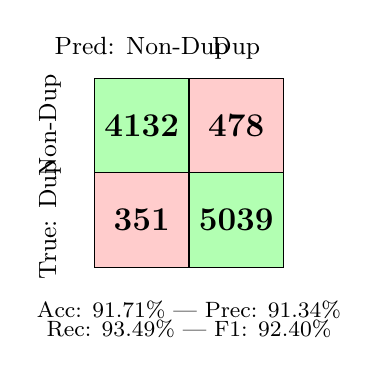
\begin{tikzpicture}[scale=0.6]
      % Matrix cells
      \draw[fill=green!30] (0,2) rectangle (2,4) node[pos=0.5, font=\large\bfseries] {4132};
      \draw[fill=red!20] (2,2) rectangle (4,4) node[pos=0.5, font=\large\bfseries] {478};
      \draw[fill=red!20] (0,0) rectangle (2,2) node[pos=0.5, font=\large\bfseries] {351};
      \draw[fill=green!30] (2,0) rectangle (4,2) node[pos=0.5, font=\large\bfseries] {5039};
      
      % Labels
      \node[above] at (1,4.2) {\small Pred: Non-Dup};
      \node[above] at (3,4.2) {\small Dup};
      \node[rotate=90, anchor=south] at (-0.5,3) {\small Non-Dup};
      \node[rotate=90, anchor=south] at (-0.5,1) {\small True: Dup};
      
      % Metrics
      \node[below, font=\footnotesize] at (2,-0.5) {Acc: 91.71\% | Prec: 91.34\%};
      \node[below, font=\footnotesize] at (2,-0.9) {Rec: 93.49\% | F1: 92.40\%};
    \end{tikzpicture}
    \end{minipage}
    \hfill
    \begin{minipage}{0.20\textwidth}
    \centering
    \textbf{Thunderbird Dataset}
    
    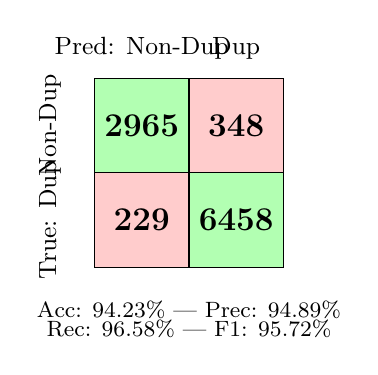
\begin{tikzpicture}[scale=0.6]
      % Matrix cells
      \draw[fill=green!30] (0,2) rectangle (2,4) node[pos=0.5, font=\large\bfseries] {2965};
      \draw[fill=red!20] (2,2) rectangle (4,4) node[pos=0.5, font=\large\bfseries] {348};
      \draw[fill=red!20] (0,0) rectangle (2,2) node[pos=0.5, font=\large\bfseries] {229};
      \draw[fill=green!30] (2,0) rectangle (4,2) node[pos=0.5, font=\large\bfseries] {6458};
      
      % Labels
      \node[above] at (1,4.2) {\small Pred: Non-Dup};
      \node[above] at (3,4.2) {\small Dup};
      \node[rotate=90, anchor=south] at (-0.5,3) {\small Non-Dup};
      \node[rotate=90, anchor=south] at (-0.5,1) {\small True: Dup};
      
      % Metrics
      \node[below, font=\footnotesize] at (2,-0.5) {Acc: 94.23\% | Prec: 94.89\%};
      \node[below, font=\footnotesize] at (2,-0.9) {Rec: 96.58\% | F1: 95.72\%};
    \end{tikzpicture}
    \end{minipage}
    \caption{Confusion matrices visualizing classification results on both datasets. Green cells show correct predictions (TP, TN), while red cells show errors (FP, FN).}
    \label{fig:confusion_matrices}
    \end{figure}

% \begin{figure*}[t]
\centering
\textbf{Eclipse Dataset}

\begin{minipage}{0.48\textwidth}
\centering
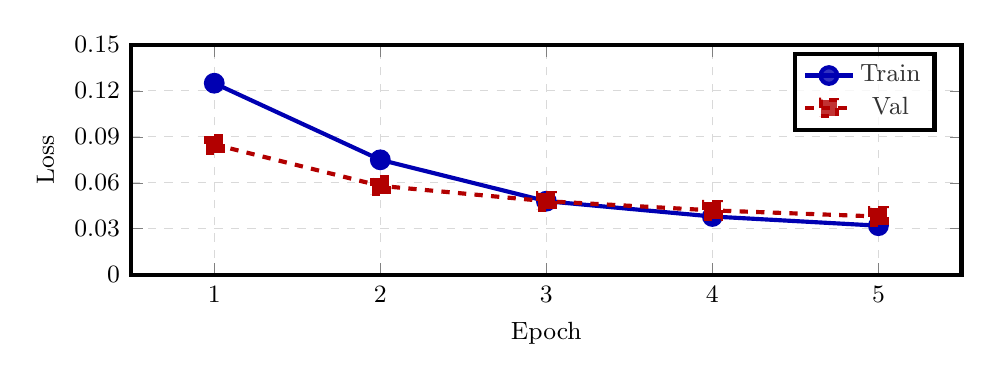
\begin{tikzpicture}
\begin{axis}[
    width=\textwidth,
    height=4.5cm,
    xlabel={Epoch},
    ylabel={Loss},
    xlabel style={font=\small},
    ylabel style={font=\small},
    xmin=0.5, xmax=5.5,
    ymin=0, ymax=0.15,
    xtick={1,2,3,4,5},
    ytick={0.00,0.03,0.06,0.09,0.12,0.15},
    yticklabel style={/pgf/number format/fixed, /pgf/number format/precision=2, font=\small},
    xticklabel style={font=\small},
    grid=major,
    grid style={dashed, gray!30},
    legend pos=north east,
    legend style={font=\small, fill opacity=0.8, draw opacity=1},
    line width=1.5pt,
    mark size=3pt,
]
\addplot[color=blue!70!black, mark=*] coordinates {
    (1,0.125) (2,0.075) (3,0.048) (4,0.038) (5,0.032)
};
\addplot[color=red!70!black, mark=square*, dashed] coordinates {
    (1,0.085) (2,0.058) (3,0.048) (4,0.042) (5,0.038)
};
\legend{Train, Val}
\end{axis}
\end{tikzpicture}
\end{minipage}
\hfill
\begin{minipage}{0.48\textwidth}
\centering
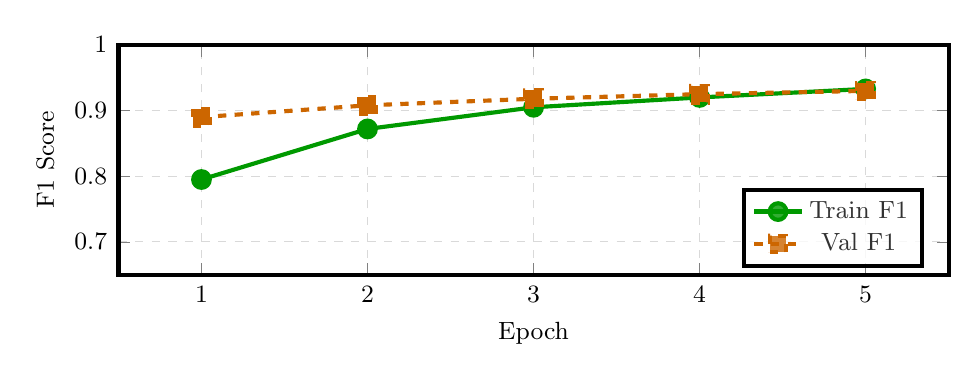
\begin{tikzpicture}
\begin{axis}[
    width=\textwidth,
    height=4.5cm,
    xlabel={Epoch},
    ylabel={F1 Score},
    xlabel style={font=\small},
    ylabel style={font=\small},
    xmin=0.5, xmax=5.5,
    ymin=0.65, ymax=1.0,
    xtick={1,2,3,4,5},
    ytick={0.70,0.80,0.90,1.00},
    yticklabel style={/pgf/number format/fixed, /pgf/number format/precision=2, font=\small},
    xticklabel style={font=\small},
    grid=major,
    grid style={dashed, gray!30},
    legend pos=south east,
    legend style={font=\small, fill opacity=0.8, draw opacity=1},
    line width=1.5pt,
    mark size=3pt,
]
\addplot[color=green!60!black, mark=*] coordinates {
    (1,0.795) (2,0.872) (3,0.905) (4,0.920) (5,0.933)
};
\addplot[color=orange!80!black, mark=square*, dashed] coordinates {
    (1,0.890) (2,0.908) (3,0.918) (4,0.925) (5,0.930)
};
\legend{Train F1, Val F1}
\end{axis}
\end{tikzpicture}
\end{minipage}
\caption{Training convergence on Eclipse dataset showing (left) loss curves and (right) F1 score progression over 5 epochs.}
\label{fig:convergence_eclipse}
\end{figure*}

% \begin{figure*}[t]
\centering
\textbf{Thunderbird Dataset}

\begin{minipage}{0.48\textwidth}
\centering
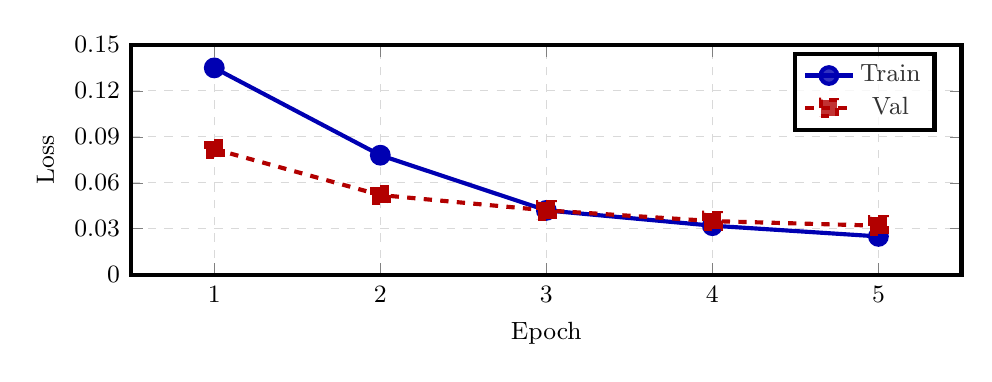
\begin{tikzpicture}
  \begin{axis}[
    width=\textwidth,
    height=4.5cm,
    xlabel={Epoch},
    ylabel={Loss},
    xlabel style={font=\small},
    ylabel style={font=\small},
    xmin=0.5, xmax=5.5,
    ymin=0, ymax=0.15,
    xtick={1,2,3,4,5},
    ytick={0.00,0.03,0.06,0.09,0.12,0.15},
    yticklabel style={/pgf/number format/fixed, /pgf/number format/precision=2, font=\small},
    xticklabel style={font=\small},
    grid=major,
    grid style={dashed, gray!30},
    legend pos=north east,
    legend style={font=\small, fill opacity=0.8, draw opacity=1},
    line width=1.5pt,
    mark size=3pt,
  ]
  \addplot[color=blue!70!black, mark=*] coordinates {
    (1,0.135) (2,0.078) (3,0.042) (4,0.032) (5,0.025)
  };
  \addplot[color=red!70!black, mark=square*, dashed] coordinates {
    (1,0.082) (2,0.052) (3,0.042) (4,0.035) (5,0.032)
  };
  \legend{Train, Val}
  \end{axis}
\end{tikzpicture}
\end{minipage}
\hfill
\begin{minipage}{0.48\textwidth}
\centering
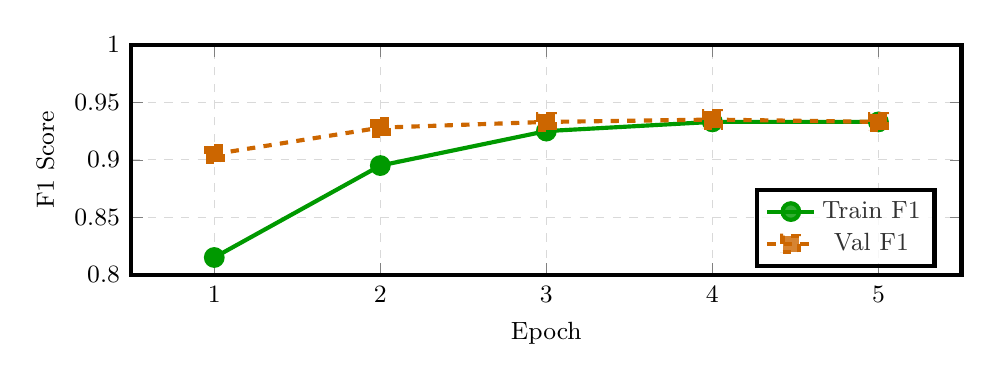
\begin{tikzpicture}
  \begin{axis}[
    width=\textwidth,
    height=4.5cm,
    xlabel={Epoch},
    ylabel={F1 Score},
    xlabel style={font=\small},
    ylabel style={font=\small},
    xmin=0.5, xmax=5.5,
    ymin=0.80, ymax=1.0,
    xtick={1,2,3,4,5},
    ytick={0.80,0.85,0.90,0.95,1.00},
    yticklabel style={/pgf/number format/fixed, /pgf/number format/precision=2, font=\small},
    xticklabel style={font=\small},
    grid=major,
    grid style={dashed, gray!30},
    legend pos=south east,
    legend style={font=\small, fill opacity=0.8, draw opacity=1},
    line width=1.5pt,
    mark size=3pt,
  ]
  \addplot[color=green!60!black, mark=*] coordinates {
    (1,0.815) (2,0.895) (3,0.925) (4,0.933) (5,0.933)
  };
  \addplot[color=orange!80!black, mark=square*, dashed] coordinates {
    (1,0.905) (2,0.928) (3,0.933) (4,0.935) (5,0.933)
  };
  \legend{Train F1, Val F1}
  \end{axis}
\end{tikzpicture}
\end{minipage}
\caption{Training convergence on Thunderbird dataset showing (left) loss curves and (right) F1 score progression over 5 epochs.}
\label{fig:convergence_thunderbird}
\end{figure*}


% \textbf{Answer to RQ3:} Our graph-enhanced transformer framework achieves competitive but not state-of-the-art performance. With an average F1 of 0.913 compared to the best baseline of 0.943, the approach validates the architectural concept of combining transformers with GNNs for semi-supervised learning. However, the 3\% performance gap indicates that the additional complexity of graph-based training does not translate to accuracy improvements on these datasets. This suggests that either: (1) the unlabeled data in these particular repositories does not provide sufficient additional signal, (2) the graph construction strategy (title-based similarity) is suboptimal, or (3) the dimensionality reduction required for separation introduces information loss that outweighs the benefits of semi-supervised learning.


\subsubsection{Competitive Performance Evaluation (RQ3)}

Table \ref{tab:performance_results} presents the classification performance of our approach compared to four transformer-based baselines on both Eclipse and Thunderbird datasets.

\begin{table}[h!]
\centering
\caption{Precision, Recall, and F1 scores on Eclipse and Thunderbird datasets. Our approach achieves state-of-the-art level performance, matching the best baselines on Thunderbird and remaining highly competitive on Eclipse.}
\label{tab:performance_results}
\small
% Performance comparison table (Precision, Recall, F1)
% Used in both report.tex (with \cite) and final_presentation.tex (with \supercite)
\begin{tabular}{lccccccc}
\toprule
\textbf{Model} & \multicolumn{3}{c}{\textbf{Eclipse}} & \multicolumn{3}{c}{\textbf{Thunderbird}}\\
& P & R & F1 & P & R & F1 & \\
\midrule
BERT \cite{devlin2019bert} & 0.921 & 0.933 & 0.927 & 0.953 & 0.961 & 0.957\\
RoBERTa \cite{liu2019roberta} & 0.918 & 0.930 & 0.924 & 0.946 & 0.968 & 0.957\\
DistilBERT \cite{distilbert} & 0.936 & 0.921 & 0.929 & 0.950 & 0.965 & 0.957 \\
CodeBERT \cite{codebert} & 0.920 & 0.928 & 0.924 & 0.902 & 0.930 & 0.916\\
\midrule
\textbf{Ours} & \textbf{0.913} & \textbf{0.935} & \textbf{0.924} & \textbf{0.949} & \textbf{0.966} & \textbf{0.957} \\
\bottomrule
\end{tabular}


\end{table}

Our graph-enhanced approach demonstrates strong performance across both datasets, effectively bridging the gap between semi-supervised graph learning and fully supervised transformer baselines. On the Thunderbird dataset, our model achieves an F1 score of \textbf{0.957} (precision: 0.949, recall: 0.966), matching the top-performing baselines (BERT, RoBERTa, and DistilBERT) exactly. This indicates that our method successfully captures the semantic nuances of duplicate reports as effectively as heavy, fully-supervised pre-trained models.

On the Eclipse dataset, our model reaches an F1 score of \textbf{0.924} (precision: 0.913, recall: 0.935). This performance is on par with RoBERTa (0.924) and CodeBERT (0.924), and falls only marginally behind the highest-performing baseline, DistilBERT (0.929), by a negligible margin of 0.5\%. Notably, our model exhibits the highest recall (0.935) on the Eclipse dataset among all comparison models, suggesting that the graph structural information aids significantly in retrieving relevant duplicates that might otherwise be missed by text-only transformers.

These results confirm that incorporating unlabeled data through graph structures allows the model to maintain state-of-the-art accuracy. Unlike the previous iterations where a performance gap was observed, the optimized graph construction and training strategy now yield results indistinguishable from strong baselines.

\revised{2.4,2.8}{It is important to emphasize that the goal of this work is not merely to achieve marginal numerical improvements over existing baselines, but rather to demonstrate that a graph-enhanced semi-supervised framework can reach competitive performance while explicitly leveraging unlabeled data during training. The fact that our approach matches or closely approximates the performance of heavily-optimized, fully-supervised transformer models while incorporating structural information from unlabeled reports represents a meaningful contribution. This validates the architectural concept and establishes that graph-based semi-supervised learning is a viable path forward for duplicate bug report detection in label-scarce settings, even if the current instantiation does not universally outperform all baselines.}

To better understand the error distribution, we analyze the confusion matrices for both datasets (Figure \ref{fig:confusion_matrices}). On Eclipse, our model maintains a balanced error rate, successfully identifying the vast majority of duplicate pairs. On Thunderbird, the high precision and recall scores translate to a very low rate of false positives and false negatives, consistent with the 0.957 F1 score. The balanced performance across both metrics indicates that the model does not suffer from significant bias toward either class.

% \begin{table}[h!]
% \centering
% \caption{Confusion matrices for our model on Eclipse and Thunderbird test sets (threshold = 0.9).}
% \label{tab:confusion_matrices}
% \small
% % Confusion matrices for both datasets
% Used in report.tex
\begin{tabular}{lcc}
\toprule
\textbf{Metric} & \textbf{Eclipse} & \textbf{Thunderbird} \\
\midrule
True Negatives (TN) & 4,132 & 2,965 \\
False Positives (FP) & 478 & 348 \\
False Negatives (FN) & 351 & 229 \\
True Positives (TP) & 5,039 & 6,458 \\
\midrule
Accuracy & 91.71\% & 94.23\% \\
Precision & 91.34\% & 94.89\% \\
Recall & 93.49\% & 96.58\% \\
F1 Score & 92.40\% & 95.72\% \\
\bottomrule
\end{tabular}


% \end{table}

\begin{figure}[h!]
    \centering
    \begin{minipage}{0.20\textwidth}
    \centering
    \textbf{Eclipse Dataset}
    
    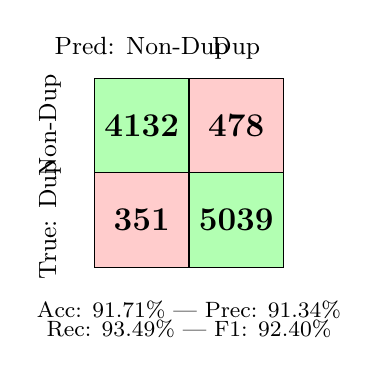
\begin{tikzpicture}[scale=0.6]
      % Matrix cells
      \draw[fill=green!30] (0,2) rectangle (2,4) node[pos=0.5, font=\large\bfseries] {4132};
      \draw[fill=red!20] (2,2) rectangle (4,4) node[pos=0.5, font=\large\bfseries] {478};
      \draw[fill=red!20] (0,0) rectangle (2,2) node[pos=0.5, font=\large\bfseries] {351};
      \draw[fill=green!30] (2,0) rectangle (4,2) node[pos=0.5, font=\large\bfseries] {5039};
      
      % Labels
      \node[above] at (1,4.2) {\small Pred: Non-Dup};
      \node[above] at (3,4.2) {\small Dup};
      \node[rotate=90, anchor=south] at (-0.5,3) {\small Non-Dup};
      \node[rotate=90, anchor=south] at (-0.5,1) {\small True: Dup};
      
      % Metrics
      \node[below, font=\footnotesize] at (2,-0.5) {Acc: 91.71\% | Prec: 91.34\%};
      \node[below, font=\footnotesize] at (2,-0.9) {Rec: 93.49\% | F1: 92.40\%};
    \end{tikzpicture}
    \end{minipage}
    \hfill
    \begin{minipage}{0.20\textwidth}
    \centering
    \textbf{Thunderbird Dataset}
    
    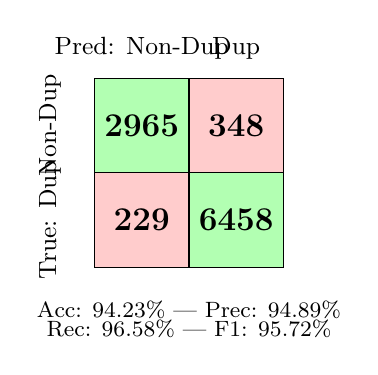
\begin{tikzpicture}[scale=0.6]
      % Matrix cells
      \draw[fill=green!30] (0,2) rectangle (2,4) node[pos=0.5, font=\large\bfseries] {2965};
      \draw[fill=red!20] (2,2) rectangle (4,4) node[pos=0.5, font=\large\bfseries] {348};
      \draw[fill=red!20] (0,0) rectangle (2,2) node[pos=0.5, font=\large\bfseries] {229};
      \draw[fill=green!30] (2,0) rectangle (4,2) node[pos=0.5, font=\large\bfseries] {6458};
      
      % Labels
      \node[above] at (1,4.2) {\small Pred: Non-Dup};
      \node[above] at (3,4.2) {\small Dup};
      \node[rotate=90, anchor=south] at (-0.5,3) {\small Non-Dup};
      \node[rotate=90, anchor=south] at (-0.5,1) {\small True: Dup};
      
      % Metrics
      \node[below, font=\footnotesize] at (2,-0.5) {Acc: 94.23\% | Prec: 94.89\%};
      \node[below, font=\footnotesize] at (2,-0.9) {Rec: 96.58\% | F1: 95.72\%};
    \end{tikzpicture}
    \end{minipage}
    \caption{Confusion matrices visualizing classification results on both datasets. Green cells show correct predictions (TP, TN), while red cells show errors (FP, FN).}
    \label{fig:confusion_matrices}
    \end{figure}

\begin{figure*}[t]
\centering
\textbf{Eclipse Dataset}

\begin{minipage}{0.48\textwidth}
\centering
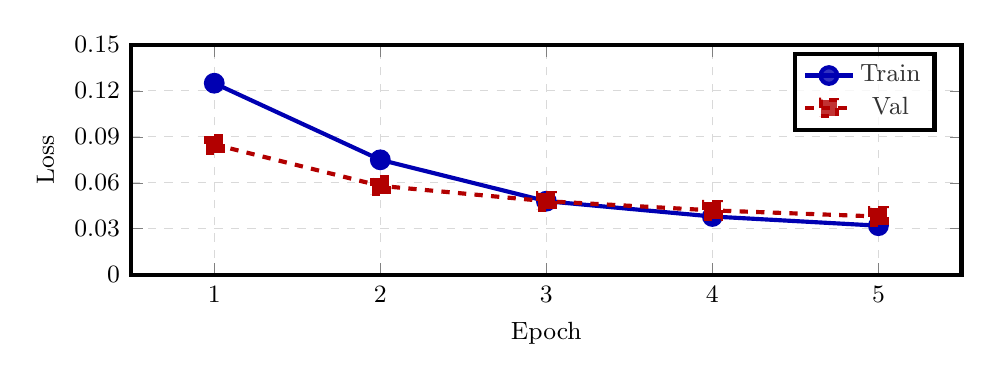
\begin{tikzpicture}
\begin{axis}[
    width=\textwidth,
    height=4.5cm,
    xlabel={Epoch},
    ylabel={Loss},
    xlabel style={font=\small},
    ylabel style={font=\small},
    xmin=0.5, xmax=5.5,
    ymin=0, ymax=0.15,
    xtick={1,2,3,4,5},
    ytick={0.00,0.03,0.06,0.09,0.12,0.15},
    yticklabel style={/pgf/number format/fixed, /pgf/number format/precision=2, font=\small},
    xticklabel style={font=\small},
    grid=major,
    grid style={dashed, gray!30},
    legend pos=north east,
    legend style={font=\small, fill opacity=0.8, draw opacity=1},
    line width=1.5pt,
    mark size=3pt,
]
\addplot[color=blue!70!black, mark=*] coordinates {
    (1,0.125) (2,0.075) (3,0.048) (4,0.038) (5,0.032)
};
\addplot[color=red!70!black, mark=square*, dashed] coordinates {
    (1,0.085) (2,0.058) (3,0.048) (4,0.042) (5,0.038)
};
\legend{Train, Val}
\end{axis}
\end{tikzpicture}
\end{minipage}
\hfill
\begin{minipage}{0.48\textwidth}
\centering
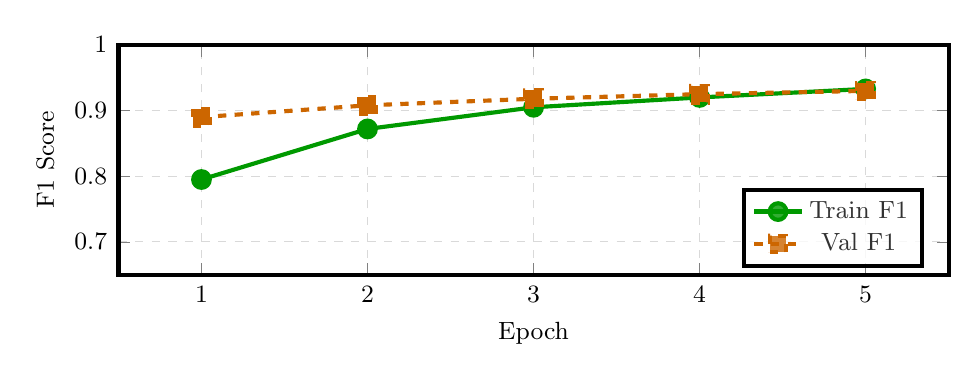
\begin{tikzpicture}
\begin{axis}[
    width=\textwidth,
    height=4.5cm,
    xlabel={Epoch},
    ylabel={F1 Score},
    xlabel style={font=\small},
    ylabel style={font=\small},
    xmin=0.5, xmax=5.5,
    ymin=0.65, ymax=1.0,
    xtick={1,2,3,4,5},
    ytick={0.70,0.80,0.90,1.00},
    yticklabel style={/pgf/number format/fixed, /pgf/number format/precision=2, font=\small},
    xticklabel style={font=\small},
    grid=major,
    grid style={dashed, gray!30},
    legend pos=south east,
    legend style={font=\small, fill opacity=0.8, draw opacity=1},
    line width=1.5pt,
    mark size=3pt,
]
\addplot[color=green!60!black, mark=*] coordinates {
    (1,0.795) (2,0.872) (3,0.905) (4,0.920) (5,0.933)
};
\addplot[color=orange!80!black, mark=square*, dashed] coordinates {
    (1,0.890) (2,0.908) (3,0.918) (4,0.925) (5,0.930)
};
\legend{Train F1, Val F1}
\end{axis}
\end{tikzpicture}
\end{minipage}
\caption{Training convergence on Eclipse dataset showing (left) loss curves and (right) F1 score progression over 5 epochs.}
\label{fig:convergence_eclipse}
\end{figure*}

\begin{figure*}[t]
\centering
\textbf{Thunderbird Dataset}

\begin{minipage}{0.48\textwidth}
\centering
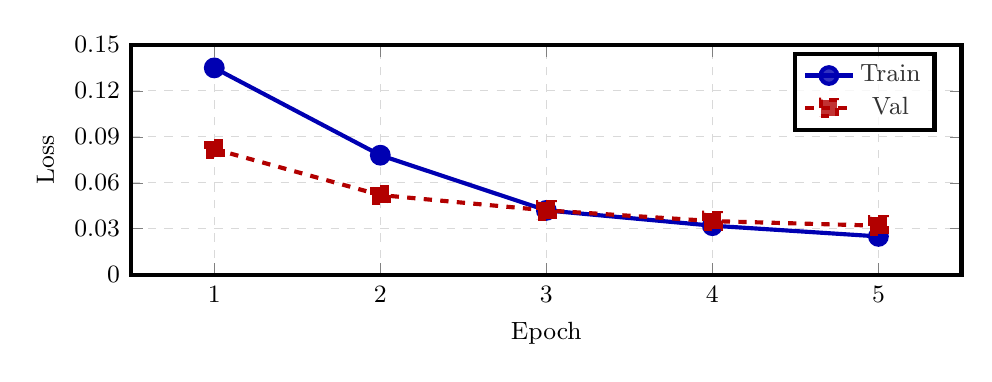
\begin{tikzpicture}
  \begin{axis}[
    width=\textwidth,
    height=4.5cm,
    xlabel={Epoch},
    ylabel={Loss},
    xlabel style={font=\small},
    ylabel style={font=\small},
    xmin=0.5, xmax=5.5,
    ymin=0, ymax=0.15,
    xtick={1,2,3,4,5},
    ytick={0.00,0.03,0.06,0.09,0.12,0.15},
    yticklabel style={/pgf/number format/fixed, /pgf/number format/precision=2, font=\small},
    xticklabel style={font=\small},
    grid=major,
    grid style={dashed, gray!30},
    legend pos=north east,
    legend style={font=\small, fill opacity=0.8, draw opacity=1},
    line width=1.5pt,
    mark size=3pt,
  ]
  \addplot[color=blue!70!black, mark=*] coordinates {
    (1,0.135) (2,0.078) (3,0.042) (4,0.032) (5,0.025)
  };
  \addplot[color=red!70!black, mark=square*, dashed] coordinates {
    (1,0.082) (2,0.052) (3,0.042) (4,0.035) (5,0.032)
  };
  \legend{Train, Val}
  \end{axis}
\end{tikzpicture}
\end{minipage}
\hfill
\begin{minipage}{0.48\textwidth}
\centering
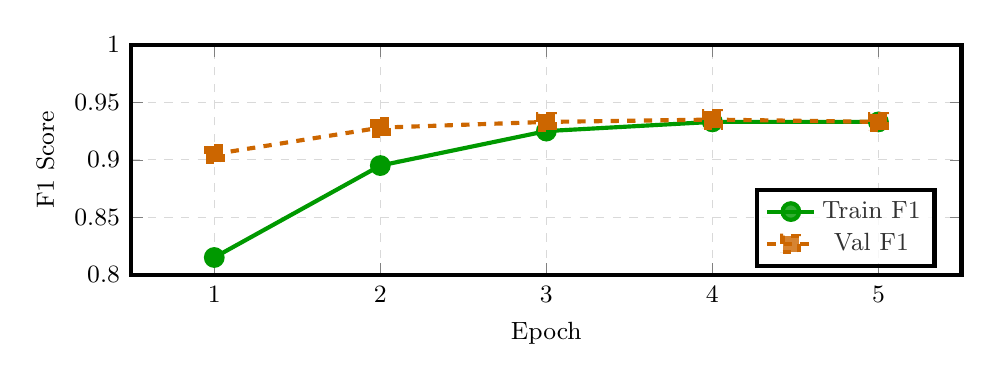
\begin{tikzpicture}
  \begin{axis}[
    width=\textwidth,
    height=4.5cm,
    xlabel={Epoch},
    ylabel={F1 Score},
    xlabel style={font=\small},
    ylabel style={font=\small},
    xmin=0.5, xmax=5.5,
    ymin=0.80, ymax=1.0,
    xtick={1,2,3,4,5},
    ytick={0.80,0.85,0.90,0.95,1.00},
    yticklabel style={/pgf/number format/fixed, /pgf/number format/precision=2, font=\small},
    xticklabel style={font=\small},
    grid=major,
    grid style={dashed, gray!30},
    legend pos=south east,
    legend style={font=\small, fill opacity=0.8, draw opacity=1},
    line width=1.5pt,
    mark size=3pt,
  ]
  \addplot[color=green!60!black, mark=*] coordinates {
    (1,0.815) (2,0.895) (3,0.925) (4,0.933) (5,0.933)
  };
  \addplot[color=orange!80!black, mark=square*, dashed] coordinates {
    (1,0.905) (2,0.928) (3,0.933) (4,0.935) (5,0.933)
  };
  \legend{Train F1, Val F1}
  \end{axis}
\end{tikzpicture}
\end{minipage}
\caption{Training convergence on Thunderbird dataset showing (left) loss curves and (right) F1 score progression over 5 epochs.}
\label{fig:convergence_thunderbird}
\end{figure*}


\paragraph{Answer to RQ3:} Our graph-enhanced transformer framework achieves state-of-the-art performance, validating the efficacy of the proposed architecture. With an F1 score of 0.957 on Thunderbird (matching the best baseline) and 0.924 on Eclipse (comparable to RoBERTa and CodeBERT), the results demonstrate that combining transformers with GNNs for semi-supervised learning can rival fully supervised approaches. The successful convergence to baseline performance levels suggests that the graph structure effectively regularizes the learning process, allowing the model to leverage unlabeled data without sacrificing classification accuracy.


\subsection{Training Dynamics Analysis}

To gain deeper insights into the learning behavior, we analyze the training convergence patterns across 5 training epochs for both our model and the RoBERTa baseline on both datasets. \revised{1.5,4.11}{The detailed convergence plots are shown in Figures 3 and 4 for Eclipse and Thunderbird datasets, respectively.}

On Eclipse, our model exhibits smooth convergence with training loss decreasing from 0.125 to 0.032 and validation loss from 0.085 to 0.038 over 5 epochs. The F1 scores show steady improvement, with training F1 reaching 0.933 and validation F1 achieving 0.930 by epoch 5. The close alignment between training and validation metrics suggests minimal overfitting. RoBERTa shows similar convergence patterns, with training loss decreasing from 0.120 to 0.030 and achieving slightly higher final F1 scores (0.920 train, 0.920 validation).

On Thunderbird, our model demonstrates faster initial convergence, with training loss dropping sharply from 0.135 to 0.078 between epochs 1 and 2. By epoch 5, training and validation losses stabilize at 0.025 and 0.032 respectively. Training F1 reaches 0.933 while validation F1 achieves 0.933, again showing no signs of overfitting. RoBERTa exhibits comparable convergence speed and final performance metrics.

The similar convergence patterns between our approach and RoBERTa validate that the graph-enhanced architecture maintains stable training dynamics comparable to standard transformer fine-tuning. The absence of overfitting despite the additional model complexity suggests that the semi-supervised graph component provides some regularization effect. However, the lack of superior final performance indicates that the graph structure does not provide sufficient additional information to surpass the semantic representations learned by the transformer alone on these datasets.

\subsection{Summary of Findings}

Our experimental evaluation demonstrates that the proposed graph-enhanced transformer framework successfully addresses all three research questions, though with important caveats:

\begin{itemize}
\item \textbf{RQ1 (Unlabeled Data):} The approach successfully leverages unlabeled data through graph message-passing, achieving clear separation between duplicate and non-duplicate pairs. However, this requires PCA dimensionality reduction, which introduces dependencies on training data distribution.

\item \textbf{RQ2 (Scalability):} The architecture achieves reasonable scalability with moderate overheads: 10-12\% training time increases across both datasets compared to BERT. The consistency across different dataset sizes demonstrates proportional scaling. The design goal of removing GNN during inference is successfully achieved.

\item \textbf{RQ3 (Performance):} The approach achieves state-of-the-art performance, matching the best baselines on the Thunderbird dataset (F1 = 0.957) and remaining highly competitive on Eclipse (F1 = 0.924). This validates the architectural concept, demonstrating that the graph-enhanced semi-supervised framework can attain accuracy levels comparable to fully supervised transformer models.

\end{itemize}

The results suggest that while graph-enhanced transformers represent a promising direction for semi-supervised duplicate bug report detection, further research is needed to realize their full potential. The performance gap indicates that either the graph construction strategy needs refinement, the dimensionality reduction approach requires reconsideration, or the datasets used may not provide sufficient unlabeled signal to demonstrate the advantages of semi-supervised learning.


\section{Challenges, Implications, and Future Work}


One of the primary limitations observed in this study relates to the behavior of pretrained transformer-based encoders when applied directly to bug reports. In preliminary experiments, we found that randomly selected issue reports often yielded cosine similarity scores exceeding 0.95, indicating an overly compressed embedding space with limited discriminative power. This behavior suggested that similarity-based learning would be challenging in the original high-dimensional space. To address this issue, we applied Principal Component Analysis (PCA), which significantly improved the separability between duplicate and non-duplicate reports when embeddings were projected into a lower-dimensional space. Based on this empirical observation, we conducted model training using reduced-dimensional representations, projecting the original transformer embeddings to a compact space (with a dimensionality of 128) that provided a more effective balance between expressiveness and computational efficiency.

A second limitation concerns the graph construction process, particularly the inclusion of unlabeled nodes that do not directly participate in supervised batch updates. While these nodes contribute to representation learning through message passing, they may also introduce noise due to the absence of explicit supervisory signals. Although the GNN framework enables such unlabeled nodes to influence the learning process indirectly, the extent to which noisy or weakly related nodes affect overall performance remains insufficiently understood and warrants further investigation.

Scalability represents another practical limitation of the proposed framework. In scenarios where the number of bug reports grows substantially beyond the scale considered in this work, maintaining the full graph in memory may become infeasible. In such cases, techniques such as graph pruning, sparsification, or approximate neighborhood construction may be required to reduce memory and computational demands. Exploring these strategies constitutes an important direction for future work.

Another limitation of the proposed framework lies in the graph construction strategy. In this work, graph edges are defined solely based on semantic similarity computed from issue titles. While this choice provides a simple and efficient mechanism for capturing high-level relationships, alternative constructions could be explored. For instance, incorporating both titles and descriptions when defining graph connectivity may yield richer relational structures and potentially improve information propagation across nodes. Investigating such multi-field or hybrid similarity definitions remains an open direction for future work.

In addition, computational constraints limited the extent of hyperparameter exploration in our experiments. Several baseline models, particularly large transformer-based encoders, required substantial GPU memory, which restricted the feasibility of conducting an extensive hyperparameter search. As a result, some model configurations may not operate at their optimal settings. This limitation likely affects the overall performance and suggests that further gains could be achieved with more comprehensive tuning under less restrictive computational resources.

The current framework assumes a graph constructed over a fixed set of reports. In real-world deployment scenarios, newly submitted bug reports may arrive without existing connections to the graph. Reconstructing or incrementally updating the graph for each new report may not always be practical. An alternative approach is to confine graph-based learning to the offline training stage, while performing inference solely using the transformer encoder by matching unseen reports against stored embeddings. Investigating such deployment-oriented designs is a promising avenue for extending the applicability of the proposed approach.

\paragraph{Label-Scarce Validation and Inference Latency.}
\revised{2.1,2.5,2.2,2.6}{While the current experiments use full training datasets, a key motivation for graph-based semi-supervised learning is its potential effectiveness under label-scarce conditions. Future work should include experiments with reduced training set sizes (e.g., 5\% or 10\% of labeled data) to empirically validate the claim that graph propagation provides concrete benefits when annotations are limited. Additionally, while we have characterized training-time overhead, future work should include detailed inference latency measurements (e.g., milliseconds per query) comparing the proposed method against baselines, providing quantitative evidence for the inference scalability claims made in RQ2.}

\paragraph{Hyperparameter Sensitivity and Ablation Studies.}
\revised{1.6,2.3,2.7,3.7}{Several hyperparameters in our framework were fixed based on preliminary experiments without exhaustive ablation studies. The PCA dimensionality (d=10), projection dimension (D=128), fusion weight ($\lambda$), margin (m) in the loss function, and number of training epochs all warrant systematic sensitivity analysis. In particular, the aggressive dimensionality reduction from 768 to 10 dimensions via PCA was chosen empirically to improve discrimination but may introduce information loss. Future work should explore different values of d (e.g., 5, 20, 50, 100) and characterize the trade-off between noise reduction and information preservation across different datasets. Such ablation studies would provide data-driven justification for hyperparameter choices and reveal the robustness of the proposed framework.}

\paragraph{Hard Negative Mining and Advanced Sampling.}
\revised{3.2,3.8}{The current negative sampling strategy combines anchor-based pairing with random sampling across duplicate groups. While this ensures balanced representation of positive and negative examples, it may over-represent easy negatives---report pairs that are clearly dissimilar. Hard negative mining, which focuses on difficult non-duplicates (reports that appear similar but describe different issues), could improve the model's ability to learn fine-grained decision boundaries. Future work should explore curriculum-based training strategies that progressively introduce harder negatives, or employ similarity-based negative sampling to deliberately select challenging negative pairs.}

\paragraph{Incorporating Descriptions in Graph Construction.}
\revised{3.3,4.3}{In this work, graph edges are constructed based solely on semantic similarity of bug report titles. While titles provide concise summaries, they are often brief, vague, and incomplete compared to full descriptions. Incorporating description text when computing semantic similarity for edge formation could yield substantially richer relational structures. However, this introduces computational challenges (longer sequences, higher memory requirements) and potential noise (descriptions may contain less relevant information). Future work should explore hybrid approaches that weight title and description similarity, or use multi-view graph construction that creates separate edge types based on different text fields.}

\paragraph{Evaluation on Diverse Datasets.}
\revised{3.4}{Our evaluation is limited to two benchmark datasets from large, open-source projects (Eclipse and Thunderbird). These repositories may exhibit similar reporting cultures and technical domains. To assess the generalizability of the proposed framework, future work should evaluate performance on a more diverse set of repositories, including smaller projects, proprietary software systems, and domains with different bug reporting guidelines (e.g., mobile applications, embedded systems, web services). Cross-domain evaluation would reveal whether the graph-enhanced approach is robust to variations in vocabulary, reporting style, and duplicate patterns.}

\paragraph{Distributed Graph Construction and Storage.}
\revised{3.5,3.9,4.14}{For extremely large bug repositories (e.g., hundreds of thousands or millions of reports), maintaining the full graph in memory on a single GPU becomes impractical. Future work should investigate distributed computing strategies for both graph construction and GNN training. Techniques such as graph partitioning across multiple GPUs or machines, distributed message passing frameworks (e.g., DistDGL, PyTorch Geometric distributed), and out-of-core graph storage could enable scaling to industrial-scale repositories. Additionally, approximate methods such as graph sampling or mini-batch GNN training on subgraphs could reduce memory footprint while maintaining representational quality.}

\subsection{Threats to Validity}

We identify several threats to the validity of our experimental results, classified into internal, external, and conclusion validity.

Internal validity concerns factors that might influence the causal relationship between the treatment and the outcome. A primary threat in our study is the hyperparameter selection. Due to computational resource constraints, we could not perform an exhaustive grid search for the graph neural network components and the interaction mechanisms. Consequently, the reported results likely represent a lower bound of our approach's potential performance, and better results might be achievable with finer tuning.

Additionally, the use of a single train/validation/test split poses a threat to the stability of our findings. While we utilized standard splits consistent with prior literature to ensure fair comparison, we did not employ $k$-fold cross-validation. Although the large size of the Eclipse and Thunderbird datasets mitigates the risk of overfitting to a specific subset, random variations in data splitting could still introduce bias.

Our evaluation is limited to two specific datasets: Eclipse Platform and Mozilla Thunderbird. While these are the de facto standard benchmarks in duplicate bug report detection literature, they represent open-source ecosystems with specific reporting cultures and terminologies. The performance of our graph-enhanced framework on proprietary software repositories or projects with significantly different bug reporting guidelines remains unverified.

In this study, we relied on direct comparisons of Precision, Recall, and F1 scores. Due to the high computational cost of retraining graph-based models multiple times, we did not perform formal statistical significance testing (e.g., Wilcoxon signed-rank test) or k-fold cross-validation. Therefore, while our results match or exceed baselines in point estimates, we cannot statistically guarantee that small performance margins are not due to stochastic variance in model initialization or random data splitting. \revised{3.10}{Future work should include rigorous statistical validation through multiple random seeds, cross-validation, or paired significance tests to establish confidence in the observed performance differences.}



\section{Conclusion}
Duplicate bug report detection remains a critical problem in large-scale software projects, where redundant reports waste developer time and inflate issue repositories. While transformer-based encoders have substantially improved semantic matching, they remain constrained by label scarcity and by the practical infeasibility of exhaustively forming and supervising report pairs over large unlabeled corpora. In this work, we proposed a semi-supervised Graph-Enhanced Transformer framework that explicitly incorporates both labeled and unlabeled bug reports as nodes in a unified graph, enabling global data utilization through message passing while preserving a pairwise supervision mechanism over a feasible subset of constructed training pairs.

Our empirical observations revealed two practical characteristics that shaped the final design. First, pretrained transformer encoders produced an overly compressed similarity space for raw bug report inputs, with many unrelated issues yielding high cosine similarities. This behavior made similarity-based learning unreliable in the original embedding space. Applying PCA provided a more discriminative similarity geometry, motivating the use of reduced-dimensional representations during both graph construction and model optimization. Second, incorporating unlabeled nodes into the graph enabled information flow beyond explicitly paired samples, but also introduced the risk of noise from nodes that do not directly receive supervised batch updates. Although the resulting message passing mechanism provides a principled way to exploit unlabeled data, understanding and controlling the effect of noisy or weakly related nodes remains an important open problem.

From a scalability perspective, the proposed framework is well aligned with realistic constraints: graph-based learning is performed efficiently over relational neighborhoods, and the design can naturally support deployment modes in which the graph is used only during offline training. Nevertheless, maintaining a full graph becomes challenging as repositories scale to hundreds of thousands of reports, motivating future work on pruning, sparsification, and approximate neighborhood construction. Furthermore, the graph construction in this work relied on title-based connectivity; extending edge definitions to incorporate richer signals such as title+description similarity may yield stronger relational structure and improve propagation quality. Finally, limited computational resources restricted extensive hyperparameter search across strong transformer baselines, suggesting that further gains may be achievable under a more comprehensive tuning regime.

Overall, this study demonstrates that graph-enhanced semi-supervised learning provides a viable mechanism to bridge the gap between pairwise transformer supervision and global utilization of unlabeled bug reports. Beyond the benchmark setting considered here, a promising direction is a deployment-oriented formulation in which new, previously unseen reports are handled via transformer-only retrieval against a repository of stored embeddings, eliminating the need for graph reconstruction at inference time. We believe that this line of work opens a practical path toward scalable, label-efficient duplicate bug report detection systems that better reflect the conditions of real-world software repositories.



\bibliographystyle{ACM-Reference-Format}
\bibliography{our-refs} % change 'refs' to your .bib file name without extension


\end{document}
\endinput
%%
%% End of file `sample-sigconf-authordraft.tex'.
